\documentclass{article}

% Título del artículo
\title{Teoría de Conjuntos}
\author{Edwin Leonel Lee Tiño}
\date{\today}

% Paquetes configurar página
\usepackage[margin=2.5cm]{geometry}
\usepackage{parskip}
\usepackage{xcolor}
\usepackage{float}

% Paquetes matemáticos
\usepackage{amsmath}
\usepackage{amssymb}
\usepackage{amsthm}

% Paquetes para gráficos
\usepackage{pgfplots}
\pgfplotsset{compat=1.18}
\usepgfplotslibrary{fillbetween}
\usepackage{tikz}
\usetikzlibrary{patterns}

% --- Inicio del documento ---
\begin{document}
\maketitle

\section{Conjunto}

Un conjunto es una colección bien definida de objetos distintos, llamados \textbf{elementos}. Por "bien definida" se debe entender que se puede decidir sin ambigüedad si un objeto dado pertenece o no a la colección.

\textit{Ejemplo:}

El conjunto de los días de la semana está bien definido. El conjunto de las "personas altas" no lo está, a menos que se fije un criterio, por ejemplo "mayores de 1.80m".

\section{Notación}

$x \in A$ que se lee "$x$ pertenece a $A$".

$x \notin A$ que se lee "$x$ no pertenece a $A$".

Un conjunto se puede definir por \textbf{extensión}, listando sus elementos:

\[A = \{1, 2, 3, 4, 5 \} \]

O por \textbf{comprensión}, describiendo una propiedad:

\[A = \{x \mid x \in \mathbb{Z}, 1 \le x \le 5  \} \]

\section{Conjuntos especiales}

\subsection{Conjunto vacío} 

El conjunto vacío cumple con:

\begin{itemize}
    \item Se representa mediante $\emptyset$ o $\{\}$. 
    \item No contiene ningún elemento.
    \item Es único (se demuestra en el apartado "6 Propiedades y demostraciones").
    \item Es subconjunto de cualquier otro conjunto.
\end{itemize}  

\subsection{Conjunto universal} 

Se representa con la letra $U$. 

Es el conjunto que contiene "todos" los elementos relevantes para un contexto particular. Su definición dependerá del problema que se esté resolviendo.

\section{Subconjuntos}

Se dice que $A$ es un subconjunto de $B$, si todo elemento de $A$ es también elemento de $B$. 

Un subconjunto está denotado por: 

\[A \subseteq B\]

Formalmente un subconjunto se define como: 

\[A \subseteq B \iff \forall x \, (x \in A \implies x \in B)\]

Se dice que $A$ es un \textbf{subconjunto propio} de $B$ si se cumple:

\[A \subseteq B \land A \neq B \implies A \subsetneq B\]

\subsection{La Paradoja de Russell}

La teoría "ingenua" de conjuntos permite formar un conjunto a partir de cualquier propiedad. Esto puede resultar en \textbf{contradicciones}. 

Si se considera la propiedad $P(x): x \notin x$ y se forma el conjunto: $R = \{ x \mid x \notin x \}$.

Se podría formular la siguiente pregunta: ¿Es $R \in R$?

Acá existen dos escenarios posibles:

\begin{itemize}
    \item Si $R \in R$, entonces por su propia definición se debe cumplir que $R \notin R$ (lo cual es una contradicción).
    \item Si $R \notin R$, entonces cumple la propiedad para estar en R, por lo tanto, $R \in R$ (nuevamente se ha llegado a una contradicción). 
\end{itemize}

Esta paradoja demostró que la teoría de conjuntos debía \textbf{axiomatizarse} para evitar tales construcciones. 

\section{Operaciones entre conjuntos}

\begin{itemize}
    \item \textbf{Unión}: Es el conjunto de todos los elementos que están en $A$, o en $B$, o en ambos.
    
    \[ A \cup B = \{x \mid x \in A \lor x \in B \} \]    
    
    \item \textbf{Intersección:} Es el conjunto de todos los elementos que están en $A$ y $B$.
    
    \[ A \cap B = \{x \mid x \in A \land x \in B  \}  \]

    \item \textbf{Diferencia:} Es el conjunto de elementos que están a $A$ pero no en $B$.
    
    \[ A - B = \{x \mid x \in A \land x \notin B  \} \]
    
    \item \textbf{Complemento:} Corresponde al conjunto de todos los elementos de $U$ que no están en un conjunto $A$.
    
    \[ A^C = \{x \mid x \in U \land x \notin A  \}  \]
\end{itemize}

\section{Propiedades y demostraciones}

No basta con conocer las operaciones de conjuntos, es necesario poder demostrar sus propiedades.

La estrategia para demostrar igualdad de conjuntos es la \textbf{doble contención}:

\[ A = B \iff  A \subseteq B \land B \subseteq A \]

\textit{Ejemplo:}

Demostrar que el conjunto $\emptyset$ es único.

Se procede mediante \textbf{contradicción}.

Se supondrá que existe otro conjunto vacío, el cual se denotará mediante $\emptyset_0$.

Entonces, se formulará la siguiente hipótesis: $\emptyset \neq \emptyset_0$.

Por la definición del \textbf{conjunto vacío} se sabe que el mismo es subconjunto de cualquier otro conjunto, por lo tanto, se puede decir que:

$\emptyset \subseteq \emptyset_0 \land \emptyset_0 \subseteq \emptyset$ 

Por doble contención se tiene: 

$\emptyset = \emptyset_0$

Esto \textbf{contradice} la hipótesis inicial sobre que $\emptyset \neq \emptyset_0$.

Por lo tanto, el conjunto $\emptyset$ es único.

$\qed$

\textit{Ejemplo:}

Demostrar que $A \cup (B \cup C) = (A \cup B) \cup C$

\textbf{Primera parte:} 

$A \cup (B \cup C) \subseteq (A \cup B) \cup C$

\underline{Hipótesis:} Sea $x \in  A \cup (B \cup C)$

Se tiene que:

$x \in A  \lor x \in (B \cup C) \implies x \in A \lor (x \in B \lor x \in C)$ 

Por asociatividad se tiene:

$(x \in A \lor x \in B) \lor x \in C \implies x \in (A \cup B) \cup C$

\textbf{Segunda parte:} 

$(A \cup B) \cup C \subseteq A \cup (B \cup C)$

\underline{Hipótesis:} Sea $x \in (A \cup B) \cup C$

Dado que:

$x \in (A \cup B) \lor x \in C \implies (x \in A \lor x \in B) \lor x \in C$

Por propiedad asociativa se tiene que:

$x \in A \lor (x \in B \lor x \in C) \implies x \in A \cup (B \cup C)$

$\qed$

\newpage
\textit{Ejemplo:}

Demostrar que $A \cup \emptyset = A$

\textbf{Primera parte:} 

$A \cup \emptyset \subseteq A$

\underline{Hipótesis:} Sea $x \in A \cup \emptyset$

Se tiene que:

$x \in A \lor x \in \emptyset$

Por definición de \textbf{conjunto vacío} se sabe que $x \in \emptyset$ es una proposición falsa.

Entonces, para que la disyunción $x \in A \lor x \in \emptyset$ sea cierta se debe cumplir necesariamente que $x \in A$.

\textbf{Segunda parte:} 

$A \subseteq A \cup \emptyset$

\underline{Hipótesis:} Sea $x \in A$

En la disyunción $x \in A \lor x \in \emptyset$, la proposición $x \in A$ es cierta por hipótesis.

Por lo tanto, la disyunción completa es cierta: $x \in A \cup \emptyset$.

$\qed$

\section{Producto cartesiano}

Es el conjunto de todos los pares ordenados $(a, b)$ donde $a \in A$ y $b \in B$.

Formalmente: 

\[A \times B = \{(a,b) \mid a \in A \land b \in B \}\]

\textit{Ejemplo:}

Si $A = \{1, 2\}$ y $B = \{x, y\}$, se tiene que:

$A \times B = \{ (1, x), (1, y), (2, x), (2, y) \}$

\subsection{Propiedad de cardinalidad:}

Si $A$ y $B$ son conjuntos finitos se tiene que:

\[ \left|A \times B\right| = \left|A\right| \times \left|B\right| \]

\section{Conjunto por partes}

También conocido como \textbf{conjunto potencia}. 

Es el conjunto de todos los subconjuntos del conjunto $A$:
 
\[ P(A) = \{X \mid X \subseteq A \} \]

\textit{Ejemplo:}

Si $A = \{1, 2\}$ entonces $P(A) = \{\emptyset, \{1\}, \{2\}, \{1, 2\} \}$

\subsection{Teorema de cardinalidad} Si $A$ es un conjunto finito con $n$ elementos, entonces $P(A)$ tiene $2^n$ elementos (la demostración se realiza en el apartado "10 Principio de inducción").

\section{Aplicaciones o funciones}

Una aplicación $f$ de un conjunto $A$ (llamado \textbf{dominio}) a un conjunto $B$ (llamado \textbf{codominio}), denotado por: $A \to B$, es una relación que asigna a cada elemento $a \in A$ un \textbf{único} elemento $b \in B$.

Formalmente:

Una función $f: A \to B$ es un subconjunto del producto cartesiano $A \times B$ que cumple con:

\begin{itemize}
    \item \textbf{Existencia:} $\forall a \in A, \exists b \in B \mid (a,b) \in f$
    \item \textbf{Unicidad:} Si $(a, b_1) \in f$ y $(a, b_2) \in f \implies b_1 = b_2$
    \item \textbf{Imagen (Rango):} Es el conjunto $\text{Im}(f) = \{b \in B \mid \exists a \in A, f(a) = b\}$
\end{itemize}

\subsection{Tipos de funciones}

\textbf{a) Inyectiva (uno a uno):} Elementos distintos del dominio tienen imágenes distintas.
    
\[f: A \to B \text{ es inyectiva si } \forall a_1, a_2 \in A (f(a_1) = f(a_2) \implies a_1 = a_2)\]

\textit{Ejemplo:}

Demostrar que $f: \mathbb{R} \to \mathbb{R}$ definida por $f(x) = 2x + 1$ es inyectiva.

Se supone que $f(a) = f(b)$, para cualesquiera $a, b \in \mathbb{R}$.

Se tiene que $2a + 1 = 2b + 1$

Por \textbf{propiedad de cancelación}: $2a = 2b \implies 2a - 2b = 0 \implies 2(a - b) = 0$

Lo anterior implica que $a - b = 0 \implies a = b$

Por lo tanto, la función $f(x)$ es inyectiva.

$\qed$

\textit{Ejemplo:}

Demostrar que $f: \mathbb{R} \to \mathbb{R}$, definida por $f(x) = x^2$ es inyectiva.

Se supondrá que $f(a) = f(b)$, para cualesquiera $a, b \in \mathbb{R}$.

Entonces, $a^2 = b^2 \implies a^2 - b^2 = 0 \implies (a - b)(a + b) = 0$

Se supone que $a$ y $b$ son distintos, por lo que $(a + b)$ debe ser cero para que se cumpla: $(a - b)(a + b) = 0$

Si se considera que $a = 1$, entonces $(1 + b) = 0 \implies b = -1$

Lo anterior implica que:

$f(1) = (1)^2 = 1$ y $f(-1) = (-1)^2 = 1$

Se puede asegurar que:

$f(a) = f(b)$ no implica necesariamente que $a = b$

Por lo tanto, la función $f(x)$ no es inyectiva.

$\qed$

\textbf{b) Sobreyectiva:} El rango cubre completamente el codominio.
    
\[f: A \to B \text{ es sobreyectiva si } \forall b \in B, \exists a \in A \mid f(a) = b\]

En otras palabras: 

\[\text{Im($f$)} = B\]

\textit{Ejemplo:}

Demostrar si la función $f: \mathbb{R} \to \mathbb{R}, f(x) = 2x + 1$ es sobreyectiva. 

PD: $\forall y \in \text{Codom($f$)} = \mathbb{R}, \exists x \in \text{Dom($f$)} = \mathbb{R}$, implica que $f(x) = y$

\underline{Hipótesis:}

Sea $y \in \text{Codom($f$)}$ arbitrario.

Demostrar que existe $x \in \text{Dom($f$)} = \mathbb{R}$, tal que:

$f(x) = y$

Se tiene que $\displaystyle 2x + 1 = y \implies x = \frac{y - 1}{2}$

Como $x$ está definida por $\displaystyle \frac{y - 1}{2}$, se observa que dicha expresión no supone restricciones a los números reales, implica que $x \in \mathbb{R} = \text{Dom($f$)}$.

Luego, se evalúa $x$ en la función $f$:

$\displaystyle f(x) = 2\Big(\frac{y - 1}{2}\Big) + 1 = y - 1 + 1 =  y$

$\qed$

\textit{Ejemplo:}

Demostrar que la función $f: \mathbb{R} \to \mathbb{R}^+ \cup \{0\}$, definida por $f(x) = x^2$ es sobreyectiva.

PD: $\forall y \in \text{Codom($f$)} = \mathbb{R}^+ \cup \{0\}, \exists x \in \text{Dom($f$)} = \mathbb{R}$, tal que $f(x) = y$.

\underline{Hipótesis:}

Dado $y \in \text{Codom($f$)}$ arbitrario.

Demostrar que existe $x \in \text{Dom($f$)} = \mathbb{R}$, tal que:

$f(x) = y$

Se sabe que $x^2 = y \implies x = \pm \sqrt{y}$

Por hipótesis, se tiene que $y \in \text{Codom($f$)}$ y $\text{Codom($f$)} = \mathbb{R}^+ \cup \{0\} \implies y \ge 0$.

Por lo tanto, $y$ está bien definida para $\sqrt{y}$, con $\sqrt{y} \ge 0$.

Luego, $x = \pm \sqrt{y}$ implica que $x$ puede ser positivo, negativo o cero, en otras palabras, $x \in \mathbb{R} = \text{Dom($f$)}$.

Evaluar $x$ en la función $f$:

$f(x) = (\pm \sqrt{y})^2 = y$

$\qed$

\textbf{c) Biyectiva:} Una función es biyectiva si es inyectiva y sobreyectiva al mismo tiempo.

\subsection{Funciones inversas y composición}

\textbf{a) Función inversa:} Una función $f: A \to B$ tiene una función inversa $f^{-1}: B \to A$, si y solo si es $f$ es una función biyectiva.

La función inversa "deshace" lo que $f$ hizo (y viceversa), es decir:

\[f(f^{-1}(x)) = x \, \text{y } f^{-1}(f(x)) = x\]

\textit{Ejemplo:}

Dada la función $f(x) = 3x - 1$

Es sabido que la función $f(x)$ es biyectiva, entonces tiene función inversa:

$\displaystyle y = 3x - 1 \implies y + 1 = 3x \implies x = \frac{y + 1}{3} \implies f^{-1}(x) = \frac{x + 1}{3}$

Evaluar $f$ en $f^{-1}$:

$\displaystyle f^{-1}(f(x)) = \frac{(3x - 1) + 1}{3} = \frac{3x}{3} = x$

También es posible evaluar $f^{-1}$ en $f$:

$\displaystyle f(f^{-1}) = 3\Big(\frac{x + 1}{3}\Big) - 1 = x + 1 - 1 = x$

$\qed$

\textit{Ejemplo:}

Demostrar si la función $f: \left[0, \infty\right) \to \left[-1, \infty\right)$, definida por $f(x) = x^2 - 1$ tiene inversa $f^{-1}$

Primero, se tiene que demostrar que la función $f$ es \textbf{biyectiva}:

a) Demostrar que $f$ es \textbf{inyectiva}:

Se supone que $f(a) = f(b); \  \forall a,b \in \left[0, \infty \right)$.

Entonces $a^2 - 1 = b^2 - 1$.

Por \textbf{propiedad de cancelación} se tiene que $a^2 = b^2 \implies a^2 - b^2 = 0 \implies (a - b)(a + b) = 0$

Como $a, b \in \left[0, \infty \right)$, implica que $a$ y $b$ son positivos o iguales que cero.

Entonces, no se puede dar que $a \neq b$, ya que el producto nunca podría ser igual que cero.

Por lo tanto, $a = b$

b) Demostrar que $f$ es \textbf{sobreyectiva}:

PD: $\forall b \in [-1, \infty), \exists a \in [0, \infty)$ tal que $f(a) = b$

\underline{Hipótesis:}

Dado $b \in [-1, \infty)$ arbitrario.

Demostrar que existe al menos un $a \in [0, \infty)$ tal que $f(a) = b$.

Se tiene que $a^2 - 1 = b \implies a = \pm \sqrt{b + 1}$.

Desestimar la parte negativa de $\pm \sqrt{b + 1}$, implica que:

$a = \sqrt{b + 1}$.

Como $b \in [-1, \infty)$, significa que $b$ está bien definida para $\sqrt{b + 1}$, con $\sqrt{b + 1} \ge 0$.  

Dado que $a = \sqrt{b + 1}$, $\sqrt{b + 1} \ge 0 \implies \sqrt{b + 1} \in [0, \infty)$, se tiene que $a \in [0, \infty)$. 

Evaluar $a$ en la función $f$:

$f(a) = (\sqrt{b + 1})^2 - 1 = b + 1 - 1 = b$

Por lo tanto, la función $f$ es sobreyectiva.

Como $f$ es inyectiva y sobreyectiva, entonces $f$ es una función \textbf{biyectiva}.

Finalmente, se concluye que $f$ tiene una función inversa:

$y = x^2 - 1 \implies y + 1 = x^2 \implies \sqrt{y + 1} = \sqrt{x^2} \implies \sqrt{y + 1} = \left|x\right| \implies x = \pm \sqrt{y + 1}$

Nuevamente, como $x \in \left[0, \infty \right)$, es necesario desestimar la parte negativa en la expresión $x = \pm \sqrt{y + 1}$, por lo tanto, la función inversa está dada por:

$f^{-1}: \left[-1, \infty \right) \to \left[0, \infty \right)$, definida por $f^{-1}(x) = \sqrt{x + 1}$

$\qed$

\begin{figure}[H]
\centering
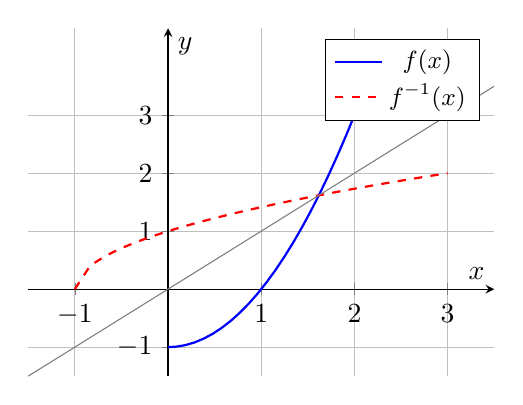
\begin{tikzpicture}
\begin{axis}[
    axis lines = middle,
    xlabel = {$x$},
    ylabel = {$y$},
    ymin=-1.5, ymax=4.5,
    xmin=-1.5, xmax=3.5,
    grid = major,
    width=7.5cm, height=6cm,
    legend pos=north east,
    legend style={font=\small},
    xtick = {-1, 0, 1, 2, 3},
    ytick = {-1, 0, 1, 2, 3}
]
% Función f(x)
\addplot [blue, thick, domain=0:2.3] {x^2 - 1};
\addlegendentry{$f(x)$}
% Función inversa
\addplot [red, thick, dashed, domain=-1:3] {sqrt(x + 1)};
\addlegendentry{$f^{-1}(x)$}
% Función identidad
\addplot [gray, thin, domain=-1.5:3.5, forget plot] {x};
\end{axis}
\end{tikzpicture}
\caption{Gráfica de la función $f(x)$ y su inversa $f^{-1}(x)$.}
\end{figure}

\textbf{b) Composición:} Sean dos funciones:

$g: A \to B$ (función interna)

$f: C \to D$ (función externa)

La \textbf{función compuesta} $(f \circ g)$ es una nueva función que va desde el dominio de la \textbf{función interna} hasta el codominio de \textbf{función externa}, si y solo si los valores que salen de la función interna pueden ser procesados por la función externa.

\textbf{Condición de existencia:} Para que $(f \circ g)$ esté bien definida se debe cumplir que:

\[ \text{Ran}(g) \subseteq \text{Dom}(f) \]

Si esto se cumple, la composición estaría dada por:

\[ (f \circ g): A \to D, \text{ definida por }(f \circ g)(x) = f(g(x)) \]

\textit{Ejemplo:}

Calcular $(f \circ g)$ para: 

$g: \mathbb{R} \to \mathbb{R}$, definida por $g(x) = x - 8$ y 

$f: \left[0, \infty \right) \to \mathbb{R}$, definida por $f(x) = \sqrt{x}$

Si $\text{Ran}(g) \subseteq \text{Dom}(f)$, entonces se cumple que:

$f \circ g: \mathbb{R} \to \mathbb{R}$ (*) 

Calcular $\text{Ran}(g):$

Sea $y \in \text{Codom}(g) = \mathbb{R}$

Por definición de rango se tiene $y = g(x) \implies y = x - 8, \forall x \in \text{Dom}(g) = \mathbb{R}$

Luego $y = x - 8 \implies x = y + 8$

Como $x = y + 8$ está definido para $\text{Dom}(g) = \mathbb{R}$, implica que $y$ está definido para todo $\mathbb{R}$.

Se puede concluir que $\text{Ran}(g) = \mathbb{R}$

Entonces, $\text{Ran}(g)= \mathbb{R} \not\subseteq \text{Dom}(f) = \left[0, \infty \right)$, implica que no se cumple (*).

Se define la función $f(g(x)) = \sqrt{x - 8}$

Como la función incluye una raíz cuadrada, el dominio está delimitado por:

$x - 8 \ge 0 \implies x \ge 8$

Por lo tanto, se tiene la función:

$f \circ g: \left[8, \infty \right) \to \mathbb{R}$, definida por $(f \circ g)(x) = \sqrt{x - 8}$

\textit{Ejemplo:}

Calcular $(f \circ g)$ para: 

$\displaystyle g: \mathbb{R} - \{0\} \to \mathbb{R} \text{, definido por } g(x) = \frac{1}{x}$ 

$\displaystyle f: \mathbb{R} - \{5\} \to \mathbb{R} \text{, definido por } f(x) = \frac{1}{x-5}$

Si se cumple que $\text{Ran}(g) \subseteq \text{Dom}(f)$, entonces:

$f \circ g: \mathbb{R} - \{0\} \to \mathbb{R} - \{5\}$ (*)

Hallar $\text{Ran}(g)$: 

Sea $y \in \text{Codom}(x) = \mathbb{R}$

Por definición de rango se tiene $\displaystyle y = g(x) \implies y = \frac{1}{x} \implies x = \frac{1}{y}, \forall x \in \mathbb{R} - \{0\}$

Se observa que $x$ no está definido cuando $y = 0$, implica que $\text{Ran}(g) = \mathbb{R} - \{0\}$

Como $\text{Ran}(g) = \mathbb{R} - \{0\} \not\subseteq \text{Dom}(f) = \mathbb{R} - \{5\}$, no se cumple (*)

Definir $\displaystyle f(g(x)) = \frac{1}{\frac{1}{x} - 5}$

Si se analiza el \textbf{denominador}, se podrán encontrar dos valores de "conflicto":

\begin{itemize}
    \item $\displaystyle x = 0 \implies f(g(0)) = \frac{1}{\frac{1}{0} - 5}$
    \item $\displaystyle x = \frac{1}{5} \implies f\Big(g\Big(\frac{1}{5}\Big)\Big) = \frac{1}{\frac{1}{\frac{1}{5}} - 5} = \frac{1}{5 - 5} = \frac{1}{0}$
\end{itemize}

El dominio de $f(g(x))$ está condicionado por $\mathbb{R} - \{0, \frac{1}{5}\}$

El codominio de $f(g(x))$ es $\mathbb{R}$

Por lo tanto: $f \circ g: \mathbb{R} - \{0, \frac{1}{5}\} \to \mathbb{R}$,  $\displaystyle (f \circ g)(x) = \frac{1}{\frac{1}{x} - 5}$

\newpage
\textit{Ejemplo:}

Calcular $(f \circ g)$ para: 

$g:\mathbb{R} \to \mathbb{R} \text{, definida por } g(x) = x^2 + 1$

$f: \left(0, \infty \right) \to \mathbb{R} \text{, definida por }f(x) = \text{ln(}x)$

Si $\text{Ran}(g) \subseteq \text{Dom}(f)$, se cumple que:

$f \circ g: \mathbb{R} \to \mathbb{R}$ (*)

Encontrar $\text{Ran}(g):$

Dado $y \in \text{Codom}(g) = \mathbb{R}$

Por definición de rango se tiene que $y = g(x) \implies y = x^2 + 1 \implies y - 1 = x^2 \implies \sqrt{x^2} = \sqrt{y - 1} \implies x = \pm \sqrt{y - 1}, \forall x \in \text{Dom}(g) = \mathbb{R}$

Se puede observar que $x$ no está definido cuando $y < 1 \implies \text{Ran}(g) = \left[1, \infty \right)$

Dado que $\text{Ran}(g) = \left[1, \infty \right) \subseteq \text{Dom}(f) = \left(0, \infty \right)$, se cumple (*)

Entonces: $f \circ g: \mathbb{R} \to \mathbb{R}$, definido por $(f \circ g)(x) = \text{ln}(x^2 + 1)$

\section{Principio de inducción}

Qué pasaría si se necesita demostrar que una propiedad es cierta para todos los números naturales: $1, 2, 3, \dots$ hasta el infinito. No es posible verificar uno por uno todos los números de $\mathbb{N}$. La \textbf{inducción} es la herramienta matemática que permite hacer exactamente eso.

Para demostrar que una proposición $P(n)$ es cierta para todo $n \ge n_0$, se consideran los siguientes pasos:

\begin{itemize}
    \item \textbf{Base de inducción:} Demostrar que $P(n_0)$ es cierta.
    \item \textbf{Hipótesis de inducción:} Asumir que $P(k)$ es cierta para un $k$ arbitrario pero fijo, donde $k \ge n_0$.
    \item \textbf{Paso inductivo:} Usando la hipótesis de inducción sobre que $P(k)$ es cierta, demostrar que $P(k + 1)$ también es verdadera.
    \item \textbf{Conclusión:} Por el \textbf{principio de inducción}, $P(n)$ es cierta para todo $n \ge n_0$.
\end{itemize}

\textit{Ejemplo}:

Demostrar por inducción que la suma de los primeros $n$ números pares es $n(n + 1)$.

\textbf{Proposicioń:} $2 + 4 + 6 + ... + 2n = n(n + 1), \forall n \in \mathbb{N}$

\textbf{1. Base de inducción:} 

Probar que la proposición es cierta para el primer elemento $(n_0 = 1)$:

$2(1) = 1(1 + 1) \implies 2 = 2$

\textbf{2. Hipótesis de inducción:}

Asumir que la proposición es cierta para el entero $k \ge n_0$:

$2 + 4 + 6 + ... + 2k = k(k + 1)$

\textbf{3. Paso inductivo:}

PD: Si la proposición es cierta para $P(k)$, entonces, también es cierta para $P(k + 1)$:

$2 + 4 + 6 + ... + 2k + 2(k + 1) = (k + 1)\left[(k + 1) + 1 \right]$

Es decir... 

$2 + 4 + 6 + ... + 2k + 2(k + 1) = (k + 1)(k + 2)$

Se sabe que: $2 + 4 + 6 + ... + 2k = k(k + 1)$, entonces:

$k(k + 1) + 2(k + 1) = (k + 1)(k + 2)$

Si se \textbf{factoriza} $k(k + 1) + 2(k + 1)$ se obtiene que $(k + 1)(k + 2)$

\textbf{4. Conclusión:} 

Se ha demostrado que:

\begin{itemize}
    \item La base de inducción $P(n_0)$ es cierta.
    \item Si $P(k)$ es cierta, entonces $P(k + 1)$ también es cierta.
\end{itemize}

Por principio de inducción, queda demostrado que la proposición inicial es cierta.

$\qed$

\textit{Ejemplo:}

Demostrar que si $A$ es un conjunto finito con $n$ elementos, entonces $P(A)$ tiene $2^n$ elementos.

\textbf{Proposición:} Si $\left| A\right| = n \implies \left|P(A)\right| = 2^n$

\textbf{1. Base de inducción:}

Se ha probado la proposición es cierta para $n_0 = 0$:

$A = \emptyset \implies P(A) = \{ \emptyset \}$

Implica que:

$\left|A\right| = 0 \implies \left|P(A)\right| = 2^0 = 1$

\textbf{2. Hipótesis de inducción:}

Se asume que la proposición es cierta para $k \ge n_0$, es decir:

$\left|A\right| = k \implies \left|P(A)\right| = 2^k$

Donde el conjunto $A = \{a_1, a_2, ..., a_k\}$

\textbf{3. Paso de inducción:}

PD: Si la hipótesis de inducción es cierta, entonces, un conjunto $A'$ con $k + 1$ elementos implica que $\left|P(A')\right| = 2^{k + 1}$

El conjunto $A'$ está dado por:

$A' = \{a_1, a_2, ..., a_k, a_{k+1}\}$

Se puede expresar al conjunto $A'$ como la unión del conjunto $A$ y el elemento $a_{k+1}$:

$A' = \{a_1, a_2, ..., a_k\} \cup \{a_{k + 1}\} = A \cup \{a_{k+1}\}$

Los subconjuntos de $A'$, que formarán al \textbf{conjunto potencia} $P(A')$, se dividen en dos tipos:

\begin{itemize}
    \item Los subconjuntos que no contienen al elemento $a_{k + 1}$, los cuales corresponden a los elementos de $P(A)$. Por \textbf{hipótesis de inducción} se sabe que que hay $2^k$ elementos para $P(A)$.

    \item Los subconjuntos que contienen al elemento $a_{k + 1}$, se forman al añadir a cada elemento de $P(A)$ el elemento $a_{k + 1}$. Lo anterior implica que hay $2^k$ elementos.
\end{itemize}

El total de subconjuntos corresponde a la cantidad de elementos de $P(A')$:

$\left|P(A')\right| = 2^k + 2^k$

Se supone que $2^k = a \implies a + a = 2a \implies 2(2^k) = 2^{k + 1}$

Entonces: $\left|P(A')\right| = 2^{k + 1}$

\textbf{4. Conclusión:}

Se ha demostrado:

\begin{itemize}
    \item La base de inducción $P(n_0)$ es cierta.
    \item Si $P(k)$ es cierta, entonces, $P(k + 1)$ también es cierta.
\end{itemize}

Por principio de inducción, queda demostrado que si $\left|A\right| = n \implies \left|P(A)\right| = 2^n$

$\qed$

\textit{Ejemplo:}

Demostrar por inducción que para todo $n \in \mathbb{N}$ (comenzando con $n_0 = 1$):

$3^{2n} - 1$ es divisible por $8$.

\textbf{Proposición:} $\forall n \in \mathbb{N}$ se cumple que $3^{2n} - 1 = 8r, \exists r \in \mathbb{N}$

\textbf{1. Base de inducción:}

Demostrar que la proposición se cumple para el primer término $n_0 = 1$:

$3^{2(1)} - 1 = 9 - 1 = 8$

\textbf{2. Hipótesis de inducción:}

Suponer que la proposición se cumple para cualquier $k \ge n_0$:

$3^{2k} - 1 = 8s, \exists s \in \mathbb{N}$

\textbf{3. Paso inductivo:}

PD: Si la hipótesis de inducción es cierta, entonces, $3^{2(k + 1)} - 1 = 8m, \exists m \in \mathbb{N}$

Dada la hipótesis de inducción $3^{2k} - 1 = 8s$:

Multiplicar $3^2$ en ambos lados de la ecuación $3^2(3^{2k} - 1) = 3^2(8s)$

Desarrollar el producto $3^{2k + 2} - 9 = 9(8s) \implies 3^{2(k + 1)} - 9 = 9(8s)$

Sumar $8$ en ambos lados de la expresión $3^{2(k + 1)} - 1 = 9(8s) + 8$

Factorizar la parte derecha de la ecuación $3^{2(k + 1)} - 1 = 8(9s + 1)$

Suponer que $m = 9s + 1 \implies 3^{2(k + 1)} - 1 = 8m$

\textbf{4. Conclusión:}

Se ha demostrado que:

\begin{itemize}
    \item La base inductiva es cierta.
    \item Si la hipótesis de inducción es cierta, entonces, la proposición también es verdadera para $k + 1$.
\end{itemize}

Por lo tanto, queda demostrado por inducción que $3^{2k} - 1$ es divisible por $8$, para todo $n \in \mathbb{N}$.

\section{Conjuntos finitos e infinitos}

\subsection{Conjuntos finitos}

Un conjunto $A$ es finito si:

\begin{itemize}
    \item $A$ es el conjunto vacío, o
    \item Puede ponerse en correspondencia \textbf{biyectiva} con el conjunto $\{1, 2, 3, \dots, n\}$, para algún número $n$.
\end{itemize}

\textit{Ejemplo:}

Como el conjunto $A = \{\text{manzana}, \, \text{pera}, \, \text{uva}\}$ puede hacer la biyección:

$1 \to \, \text{manzana}$

$2 \to \, \text{pera}$

$3 \to \, \text{uva}$

El conjunto $A$ es \textbf{finito} con cardinalidad = $3$.

\textbf{Propiedad:} Si $A$ es un conjunto finito, su cardinalidad $\left|A\right|$ es un número $n$ único.

\subsection{Conjuntos infinitos}

Un conjunto $A$ es infinito si no es finito. Es decir, un conjunto $A$ es infinito si no existe ningún número $n$ tal que $A$ esté en correspondencia biyectiva con el conjunto $\{1, 2, 3, ..., n\}$.

Para comparar "tamaños" de conjuntos infinitos, no se puede contar. Por lo tanto, se utilizan \textbf{biyecciones}:

\begin{itemize}
    \item Dos conjuntos $A$ y $B$ tienen la misma cardinalidad, es decir $\left|A\right| = \left|B\right|$, si existe una biyección entre dichos conjuntos.
    \item Se dice que $\left|A\right| < \left|B\right|$ si $A$ es biyectable con un subconjunto propio de $B$, pero $B$ no es biyectable con ningún subconjunto propio de $A$.
\end{itemize}

\subsection{Conjuntos numerables}

Un conjunto es \textbf{numerable} si existe una biyección con el conjunto de los números naturales $\mathbb{N}$. Esto significa que es posible "listar" sus elementos, aunque la lista nunca termine.

\textbf{Cardinalidad Aleph cero}: 

Es el nombre para denotar el tamaño de los conjuntos numerables.

Un conjunto $A$ tiene cardinalidad $\aleph_0$, si y solo si existe una biyección entre dicho conjunto y el conjunto de los números naturales $\mathbb{N}$ (es decir, es un conjunto numerable).

El subíndice cero indica que es el infinito más pequeño que existe. No hay ningún conjunto infinito que tenga menos elementos que los naturales.

\textit{Ejemplo:}

Demostrar si el conjunto de naturales $\mathbb{N}$ tiene la misma cardinalidad que el conjunto de números pares positivos $P$.

Definir la función $f: \mathbb{N} \to P, f(n) = 2n$

Dicha función recibe números naturales y "genera" números pares positivos.

a) Demostrar si la función es \textbf{inyectiva:}

Suponer que $f(a) = f(b), \forall a, b \in \text{Dom}(f) = \mathbb{N}$, entonces:

$2a = 2b \implies 2a - 2b = 0 \implies 2(a - b) = 0$

Lo anterior significa necesariamente que $a - b = 0 \implies a = b$

Por lo tanto, la función $f$ es inyectiva.

b) Demostrar si la función es \textbf{sobreyectiva:}

PD: $\forall b \in \text{Codom($f$)} = P, \exists a \in \text{Dom($f$)} = P$, tal que $f(a) = b$.

\newpage
\underline{Hipótesis:}

Sea $b \in \text{Codom($f$)}$ arbitrario.

Demostrar que existe $a \in \text{Dom($f$)}$, tal que $f(a) = b$

Se sabe que $\displaystyle 2a = b \implies a = \frac{b}{2}$

Dado que $b \in \text{Codom($f$)} = P$, entonces $b = 2k$, con $k \in \mathbb{N}$.

Por lo tanto, $\displaystyle a = \frac{b}{2} \implies \frac{2k}{2} = k \implies a \in \mathbb{N} = \text{Dom($f$)}$.

Evaluar $a$ en la función $f$:

$\displaystyle f(a) = 2\Big(\frac{b}{2}\Big) = b$

Entonces, la función $f$ es sobreyectiva.

Dado (a) y (b), se concluye que $f$ es \textbf{biyectiva}.

Se pueden generar varias conclusiones:

\begin{itemize}
    \item $\left|\mathbb{N}\right| = \left|P\right|$.
    \item Como existe una biyección entre el conjunto $P$ con el conjunto de números naturales, se puede decir que $P$ es un conjunto numerable.
    \item Por el punto anterior, se sabe que el conjunto $P$ tiene cardinalidad $\aleph_0$.
\end{itemize}

$\qed$

\textit{Ejemplo:}

Demostrar si el conjunto de los naturales $\mathbb{N}$ tiene la misma cardinalidad que el conjunto de los enteros $\mathbb{Z}$.

Definir la función: $f: \mathbb{N} \to \mathbb{Z}$, dada por:

$
f(n) = 
\begin{cases}
    \frac{n}{2} \, \text{si n es par} \\
    -\frac{n + 1}{2} \, \text{si n es impar} 
\end{cases}
$

a) Demostrar si $f$ es \textbf{inyectiva}:

\underline{Caso No. 1:} 

Considerando $a, b \in \text{Dom}(f) = \mathbb{N}$, siendo éstos números pares.

Suponer que $f(a) = f(b)$, entonces:

$\displaystyle \frac{a}{2} = \frac{b}{2} \implies \frac{a}{2} - \frac{b}{2} = 0 \implies \frac{a - b}{2} = 0 \implies \Big(\frac{1}{2}\Big)(a - b) = 0$

Implica inevitablemente que $a - b = 0 \implies a = b$

Cuando $a$ es par se tiene que:

$\displaystyle f(0) = \frac{0}{2} = 0$

$\displaystyle f(2) = \frac{2}{2} = 1$

$\displaystyle f(4) = \frac{4}{2} = 2$

$\displaystyle f(6) = \frac{6}{2} = 3$

$\displaystyle \dots$

Se puede observar que cuando $a$ es par, las imágenes serán los enteros positivos, incluyendo al cero.

\underline{Caso No. 2:} 

Tomar en cuenta que $a, b \in \text{Dom}(f) = \mathbb{N}$, siendo éstos números impares.

Nuevamente suponer que $f(a) = f(b)$, entonces:

$\displaystyle -\frac{a + 1}{2} = -\frac{b + 1}{2} \implies \frac{a + 1}{2} = \frac{b + 1}{2} \implies \frac{a + 1}{2} - \frac{b + 1}{2} = 0 \implies \frac{a + 1 -(b + 1)}{2} = 0 \implies \frac{a - b}{2} = 0 \implies \Big(\frac{1}{2}\Big)(a - b) = 0$

Implica que $a - b = 0 \implies a = b$

Cuando $a$ es impar se tiene:

$\displaystyle f(1) = -\frac{1 + 1}{2} = -1$

$\displaystyle f(3) = -\frac{3 + 1}{2} = -2$

$\displaystyle f(5) = -\frac{5 + 1}{2} = -3$

$\displaystyle f(7) = -\frac{7 + 1}{2} = -4$

$\dots$

Cuando $a$ es un número impar, las imágenes corresponden a los enteros negativos.

\underline{Caso No. 3:} 

\textbf{Caso cruzado}, donde se supone que $a$ es par y $b$ impar (o viceversa), con $a, b \in \text{Dom}(f) = \mathbb{N}$

Para el caso cruzado, no es posible que cuando $f(a) = f(b)$ implique que $a = b$. Esto se debe a que si $a$ es par, entonces $f(a) \ge 0$, mientras que si $b$ es impar, entonces $f(b) < 0$.

Esto asegura que ningún $n$ par generará una imagen correspondiente a una $n$ impar, y viceversa.

Por las demostraciones en los casos anteriores, es posible concluir que la función $f$ es inyectiva.

b) Demostrar si $f$ es \textbf{sobreyectiva}:

\underline{Caso No. 1:} 

Suponiendo cualquier $b \ge 0$.

PD: $\forall b \in \text{Codom($f$)} = \mathbb{Z} \text{ con } b \ge 0, \exists a \in \text{Dom($f$)} = \mathbb{N}$, tal que $f(a) = b$.

\underline{Hipótesis:}

Sea $b \in \text{Codom($f$)}$ arbitrario, con la única condición que sea mayor o igual que cero.

Demostrar que existe al menos un $a \in \text{Dom($f$)}$, tal que $f(a) = b$.

Entonces, se tiene $\displaystyle \frac{a}{2} = b \implies a = 2b$.

Como $a = 2b$ y $b \ge 0$, implica que $a$ es un número par positivo, significa que $a \in \mathbb{N}$.

Evaluar $a$ en la función $f$:

$\displaystyle f(a) = \frac{(2b)}{2} = b$

\underline{Caso No. 2:} 

Ahora se supondrá cualquier $b < 0$.

PD: $\forall b \in \text{Codom($f$)} = \mathbb{Z} \text{ con } b < 0, \exists a \in \text{Dom($f$)} = \mathbb{N}$.

\underline{Hipótesis:}

Dado $b \in \text{Codom($f$)}$ arbitrario, con la única condición que $b < 0$.

Demostrar que $a \in \text{Dom($f$)}$, tal que $f(a) = b$.

Se tiene que $\displaystyle -\frac{a + 1}{2} = b \implies a = -2b - 1$.

Como $b \in \text{Codom($f$)} = \mathbb{Z} \ \land \ b < 0 \implies - 2b - 1 > 0 \ \land \ -2b - 1 \text{ es impar, por lo tanto, } a \in \mathbb{N}$.

Evaluar $a$ en la función $f$:

$\displaystyle f(a) = -\frac{(-2b - 1) + 1}{2} = -\frac{-2b}{2} = -(-b) = b$

Debido a los dos casos anteriores, se observa que para cualquier $b \in \mathbb{Z}$ (se cubrieron enteros negativos, cero y positivos), existe $a \in \mathbb{N}$ (se consideraron los naturales pares e impares), tal que $f(a) = b$.

Entonces, $f$ es sobreyectiva.

Por lo tanto, $f$ es biyectiva.

De lo anterior, se concluye que:

\begin{itemize}
    \item $\left|\mathbb{N}\right| = \left|\mathbb{Z}\right|$.
    \item El conjunto de números enteros $\mathbb{Z}$ es un conjunto numerable.
    \item Por el punto anterior, se tiene que la cardinalidad de $\mathbb{Z}$ es $\aleph_0$.
\end{itemize}

$\qed$

\textit{Ejemplo:}

Demostrar si la cardinalidad del conjunto $\mathbb{N}$ es igual a la cardinalidad de $\mathbb{Q}$.

Se realizará la demostración mediante la \textbf{Diagonal de Cantor}:

\begin{table}[H]
\centering
\renewcommand{\arraystretch}{1.5}
\begin{tabular}{c|cccccc}
$n$ & 1 & 2 & 3 & 4 & 5 & $\dots$ \\ \hline
1 & \color{red}$\frac{1}{1}$ & $\frac{1}{2}$ & $\frac{1}{3}$ & $\frac{1}{4}$ & $\frac{1}{5}$ & $\dots$ \\
2 & $\frac{2}{1}$ & \color{red}$\frac{2}{2}$ & $\frac{2}{3}$ & $\frac{2}{4}$ & $\frac{2}{5}$ & $\dots$ \\
3 & $\frac{3}{1}$ & $\frac{3}{2}$ & \color{red}$\frac{3}{3}$ & $\frac{3}{4}$ & $\frac{3}{5}$ & $\dots$ \\
4 & $\frac{4}{1}$ & $\frac{4}{2}$ & $\frac{4}{3}$ & \color{red}$\frac{4}{4}$ & $\frac{4}{5}$ & $\dots$ \\
5 & $\frac{5}{1}$ & $\frac{5}{2}$ & $\frac{5}{3}$ & $\frac{5}{4}$ & \color{red}$\frac{5}{5}$ & $\dots$ \\
$\vdots$ & $\vdots$ & $\vdots$ & $\vdots$ & $\vdots$ & $\vdots$
\end{tabular}
\caption{Diagonal de Cantor ($\mathbb{Q}^+$)}
\end{table}

Si se recorre la matriz en \textbf{diagonales zigzag}, es posible elegir números racionales positivos cuya representación son fracciones, donde su numerador y denominador son \textbf{coprimos}, es decir, su \textbf{MCD} es $1$.
 
$k = 1 \implies f^+(1) = \frac{1}{1} = 1$

$k = 2 \implies f^+(2) = \frac{2}{1} = 2$

$k = 3 \implies f^+(3) = \frac{1}{2}$

$k = 4 \implies f^+(4) = \frac{3}{1} = 3$

$k = 5 \implies f^+(5) = \frac{1}{3}$

$k = 6 \implies f^+(6) = \frac{4}{1} = 4$

$k = 7 \implies f^+(7) = \frac{3}{2}$

$k = 8 \implies f^+(8) = \frac{2}{3}$

$k = 9 \implies f^+(9) = \frac{1}{4}$

$\dots$

Lo anterior implica que se puede formar:

\begin{itemize}
    \item El conjunto $L^+ = \{1, 2, \frac{1}{2}, 3, \frac{1}{3}, 4, \frac{3}{2}, \frac{2}{3}, \frac{1}{4}, \dots\}$
    \item La biyección $f^+ : \mathbb{N} \to \mathbb{Q^+}$, definida por $f^+(k)$, donde $k \ge 0$
\end{itemize}

Ahora, se forma la matriz que permita generar los racionales negativos:

\begin{table}[H]
\centering
\renewcommand{\arraystretch}{1.5}
\begin{tabular}{c|cccccc}
$n$ & 1 & 2 & 3 & 4 & 5 & $\dots$ \\ \hline
-1 & \color{red}$-\frac{1}{1}$ & $-\frac{1}{2}$ & $-\frac{1}{3}$ & $-\frac{1}{4}$ & $-\frac{1}{5}$ & $\dots$ \\
-2 & $-\frac{2}{1}$ & \color{red}$-\frac{2}{2}$ & $-\frac{2}{3}$ & $-\frac{2}{4}$ & $-\frac{2}{5}$ & $\dots$ \\
-3 & $-\frac{3}{1}$ & $-\frac{3}{2}$ & \color{red}$-\frac{3}{3}$ & $-\frac{3}{4}$ & $-\frac{3}{5}$ & $\dots$ \\
-4 & $-\frac{4}{1}$ & $-\frac{4}{2}$ & $-\frac{4}{3}$ & \color{red}$-\frac{4}{4}$ & $-\frac{4}{5}$ & $\dots$ \\
-5 & $-\frac{5}{1}$ & $-\frac{5}{2}$ & $-\frac{5}{3}$ & $-\frac{5}{4}$ & \color{red}$-\frac{5}{5}$ & $\dots$ \\
$\vdots$ & $\vdots$ & $\vdots$ & $\vdots$ & $\vdots$ & $\vdots$
\end{tabular}
\caption{Diagonal de Cantor ($Q^-$)}
\end{table}

Nuevamente se recorre la matriz mediante movimientos diagonales zigzag, para seleccionar racionales negativos, en forma de fracciones con numeradores y denominadores coprimos:

$k = 1 \implies f^-(1) = -\frac{1}{1} = -1$

$k = 2 \implies f^-(2) = -\frac{2}{1} = -2$

$k = 3 \implies f^-(3) = -\frac{1}{2}$

$k = 4 \implies f^-(4) = -\frac{3}{1} = -3$

$k = 5 \implies f^-(5) = -\frac{1}{3}$

$k = 6 \implies f^-(6) = -\frac{4}{1} = -4$

$k = 7 \implies f^-(7) = -\frac{3}{2}$

$k = 8 \implies f^-(8) = -\frac{2}{3}$

$k = 9 \implies f^-(9) = -\frac{1}{4}$

$\dots$

Entonces, es posible formar:

\begin{itemize}
    \item El conjunto $L^- = \{-1, -2, -\frac{1}{2}, -3, -\frac{1}{3}, -4, -\frac{3}{2}, -\frac{2}{3}, -\frac{1}{4}, \dots\}$
    \item La biyección $f^- : \mathbb{N} \to \mathbb{Q^-}$, definida por $f^-(k)$, con $k \ge 0$
\end{itemize}

Crear un nuevo conjunto $L = L^+ \cup L^- \cup \{0\}$

Dividir los números naturales en pares e impares, definiendo:

\begin{itemize}
    \item Si $n$ es par, entonces $n = 2k \implies k = \frac{n}{2}$
    \item Si $n$ es impar, entonces $n = 2k + 1 \implies k = \frac{n - 1}{2}$
\end{itemize}

Luego, se crea la biyección:

$f: \mathbb{N} \to \mathbb{Q}$, definida por:

$
f(n) = 
\begin{cases}
    0 \, \text{si } n = 1 \\
    f^+(k) = f^+(\frac{n}{2}) \, \text{ si } n \in 2 \mathbb{N}, n \ge 2 \\
    f^-(k) = f^-(\frac{n - 1}{2}) \, \text{si } n \in 2 \mathbb{N} + 1, n \ge 3
\end{cases}
$

Se tiene que:

$f(1) = 0$

$f(2) = f^+(\frac{2}{2}) = f^+(1) = 1$

$f(3) = f^-(\frac{3 - 1}{2}) = f^-(1) = -1$

$f(4) = f^+(\frac{4}{2}) = f^+(2) = 2$

$f(5) = f^-(\frac{5 - 1}{2}) = f^-(2) = -2$

$f(6) = f^+(\frac{6}{2}) = f^+(3) = \frac{1}{2}$

$f(7) = f^-(\frac{7 - 1}{2}) = f^-(3) = -\frac{1}{2}$

$\dots$

Queda demostrado que:

\begin{itemize}
    \item $\left|\mathbb{N}\right| = \left|\mathbb{Q}\right|$
    \item El conjunto de números racionales $\mathbb{Q}$ es numerable.
    \item La cardinalidad de $\mathbb{Q}$ es $\aleph_0$.
\end{itemize}

$\qed$

\subsection{Conjuntos no numerables}

Un conjunto es \textbf{no numerable} si es infinito pero no es numerable. Es decir, el conjunto tiene "más" elementos que el conjunto $\mathbb{N}$.

\textit{Ejemplo:}

Demostrar que el intervalo $(0, 1)$ no es numerable.

Para la demostración se utilizará nuevamente la \textbf{diagonal de Cantor}.

Suponer que el intervalo $(0, 1)$ es numerable, lo cual implica que:

\begin{itemize}
    \item Existe una \textbf{biyección} entre $\mathbb{N}$ y $(0, 1)$, es decir, es posible listar todos los números reales del intervalo en una secuencia infinita: $(0, 1) = \{r_1, r_2, r_3, ...\}$
    \item Escribir cada número de la lista en su expansión decimal infinita (añadiendo ceros si es necesario). Para evitar ambigüedades se asumirán representaciones que no terminen en una sucesión infinita de nueves (como 0.24999... = 0.25).
\end{itemize}

Entonces:

$r_1 = 0.d_{11}d_{12}d_{13}...$

$r_2 = 0.d_{21}d_{22}d_{23}...$

$r_3 = 0.d_{31}d_{32}d_{33}...$

$\dots$

Donde cada $d_{ij}$ es un dígito entre $0$ a $9$.

Se puede generar un número real conocido como el \textbf{número de Cantor}:

$X = 0.x_1x_2x_3...$

De tal manera que cada dígito $x_i$ es distinto al dígito de la diagonal de la lista $d_{ij}$.

Una regla sencilla para construir los dígitos de $X$ sería:

$
x_i = 
\begin{cases}
    4 \, \text{si } d_{ii} \neq 4 \\
    5 \, \text{si } d_{ii} = 4
\end{cases}
$

Esto asegura que:

\begin{itemize}
    \item $r_1 \neq X$, ya que $x_1 \neq d_{11}$
    \item $r_2 \neq X$, ya que $x_2 \neq d_{22}$
    \item $r_3 \neq X$, ya que $x_3 \neq d_{33}$
    \item $\dots$
\end{itemize}

Entonces, se ha generado una \textbf{contradicción}, ya que no se ha sido capaz de "listar" el número de Cantor en el listado $\{r_1, r_2, r_3, \dots\}$.

Por lo tanto, se puede concluir que $\left|\mathbb{N}\right| < \left|(0, 1)\right|$

$\qed$

\subsection{Teorema de Cantor}

Es un \textbf{teorema general} que dice que cualquier conjunto $A$, sea finito o infinito, tiene una cardinalidad estrictamente menor que su conjunto potencia $P(A)$.

Formalmente:

\[\text{Para cualquier conjunto } A \text{ se cumple que } \left|A\right| < \left|P(A)\right|\]

\textbf{Demostración:}

Para demostrar que $\left|A\right| < \left|P(A)\right|$ es necesario probar que no existe ninguna función sobreyectiva entre ellos.

Suponer que existe una función $f: A \to P(A)$, tal que $f$ es sobreyectiva.

Implica que para todo subconjunto $S \subseteq A$, existe al menos un elemento $a \in A$, tal que $f(a) = S$.

Luego, definir un subconjunto especial $B \subseteq A$ (llamado el \textbf{conjunto de Russell}):

$B = \{x \in A \mid x \notin f(x)\}$

Como se hizo la suposición de que $f$ es sobreyectiva, debe existir al menos un elemento $b \in A$ que sea preimagen del subconjunto $B$:

$f(b) = B$

Se formula la siguiente pregunta: ¿b pertenece a B?

Hay dos caminos posibles:

\begin{itemize}
    \item Si $b \in B \implies b \notin f(b)$, pero como $f(b) = B \implies b \notin B$ (se ha llegado a una contradicción).
    \item Si $b \notin B \implies b \in f(b)$, pero como $f(b) = B \implies b \in B$ (nuevamente, se generó una contradicción).
\end{itemize}

En ambos casos se llegó a una \textbf{contradicción}, implica que la suposición inicial ($f$ es una función sobreyectiva) es falsa, entonces, no existe biyección entre los conjuntos.

Por lo tanto, se concluye que $\left|A\right| \neq \left|P(A)\right|$

Además, como siempre existe una función inyectiva natural de $A$ hacia $P(A)$ (asignando cada elemento $a$ al conjunto unitario $\{a\}$), pero no existe una función sobreyectiva, se concluye que $\left|A\right| < \left|P(A)\right|$.

$\qed$

\textit{Ejemplo:}

Demostrar que el conjunto potencia de los números naturales, denotado como $P(\mathbb{N})$, no es un \textbf{conjunto numerable}.

Recordar la definición de conjunto numerable: "Un conjunto $A$ es numerable si existe una \textbf{biyección} con el conjunto de números naturales $\mathbb{N}$".

Suponer que existe la función $f: \mathbb{N} \to \mathbb{P(\mathbb{N})}$, la cual es sobreyectiva, entonces $\left|\mathbb{N}\right| = \left|P(\mathbb{N})\right|$.

Implica que para cualquier subconjunto $S \subseteq \mathbb{N}$, existe al menos un elemento $n \in \mathbb{N}$, tal que $f(n) = S$.

Luego, definir un subconjunto especial $B \subseteq \mathbb{N}$, conocido como el conjunto Russell:

$B = \{n \in \mathbb{N} \mid n \notin f(n)\}$

Como se tiene el supuesto de que la función $f$ es sobreyectiva, debe existir al menos un elemento $b \in \mathbb{N}$ que sea pre-imagen de $B$:

$f(b) = B$

Se formula la pregunta: ¿$b$ pertenece a $B$?

Existen dos opciones:

\begin{itemize}
    \item Si $b \in B \implies b \notin f(b)$, pero es sabido que $f(b) = B \implies b \notin B$ (se ha generado una contradicción).
    \item Si $b \notin B \implies b \in f(b)$, sin embargo, recordar que $f(b) = B \implies b \in B$ (nuevamente, se ha llegado a una contradicción).
\end{itemize}

Como en ambos casos se llegó a contradicciones, implica que la suposición inicial ($f$ es una función sobreyectiva) es falsa.

Esto permite concluir, en primera instancia, que $\left|\mathbb{N}\right| \neq \left|P(\mathbb{N})\right|$.

Adicionalmente, se sabe que existe una función inyectiva natural de $\mathbb{N}$ a $P(\mathbb{N})$ (se asigna cada elemento $n \in \mathbb{N}$ al conjunto unitario $\{n\}$), pero no existe una función sobreyectiva, se puede concluir que $\left|\mathbb{N}\right| < \left|P(\mathbb{N})\right|$.

$\qed$

\section{Familia de conjuntos}

Sea $I$ un conjunto no vacío, al cual se conoce como \textbf{conjunto de índices}. Una familia de conjuntos indexada por $I$ es una aplicación $f$ que asigna a cada elemento $i \in I$ un conjunto $A_i$.

Se denota esta colección como:

\[ \mathcal{A} = \{A_i\}_{i \in I} \]

\textit{Ejemplo:}

Definir el conjunto de índices como $I = \{1, 2, 3\}$

Luego, la regla de asignación será: Para cada $n \in I$, el conjunto $D_n$ contiene los divisores positivos para dicho número.

Formalmente:

Sea $I = \{1, 2, 3\}$, la familia $\{D_n\}_{n \in I}$ está definida por:

$D_1 = \{1\}$

$D_2 = \{1, 2\}$

$D_3 = \{1, 2, 3 \}$

\textit{Ejemplo:}

Definir formalmente la familia de conjuntos $\{C_r\}_{r \in I}$. 

Dicha familia representa a todos los círculos en el plano cartesiano que tienen su centro en el origen. Además, su radio es un número entero positivo menor o igual que $10$.

Sea $I = \{r \in \mathbb{Z} \mid 0 < r \le 10 \}$, la familia $\{C_r\}_{r \in I}$ está definida por:

$C_r = \{(x, y) \in \mathbb{R}^2 \mid x^2 + y^2 = r^2\}$

Se puede desglosar la familia de la siguiente manera:

$C_1 = x^2 + y^2 = 1^2$

$C_2 = x^2 + y^2 = 2^2$

$C_3 = x^2 + y^2 = 3^2$

\textit{Ejemplo:}

Representar los múltiplos de los primeros cinco números primos.

Definir la familia de conjuntos $\{M_p\}_{p \in I}$ tal que cada conjunto contenga los múltiplos naturales de $p$.

Dado el conjunto $I = \{2, 3, 5, 7, 11\}$, la familia de conjuntos $\{M_p\}_{p \in I}$ se define por la regla:

$M_p = \{np \mid n \in \mathbb{N}\}$

Se puede desglosar la familia como:

$M_2 = \{2, 4, 6, 8, 10, \dots\}$

$M_3 = \{3, 6, 9, 12, 15, \dots\}$

$M_5 = \{5, 10, 15, 20, 25, \dots\}$

$M_7 = \{7, 14, 21, 28, 35, \dots\}$

$M_{11} = \{11, 22, 33, 44, 55, \dots\}$

\textit{Ejemplo:}

Definir la familia de conjuntos $\{I_x\}_{x \in I}$, donde cada conjunto es un intervalo cerrado que comienza en $0$ y termina en un número real $x$, donde $x$ puede ser cualquier valor en el intervalo abierto $(0, 5)$.

Dado el conjunto $I = \{x \in \mathbb{R} \mid 0 < x < 5\}$, la familia de de conjuntos $\{I_x\}_{x \in I}$ se define mediante la regla:

$I_x = \{y \in \mathbb{R} \mid 0 \le y \le x\} = \left[0, x\right]$

\textit{Ejemplo:}

Sea $S = \{1, 2, 3\}$. 

Definir una familia $\{A_X\}_{X \in I}$, donde el conjunto de índices es el conjunto potencia de S.

La regla de asignación es: $A_X$ es el conjunto de los complementos de $X$ con respecto a $S$.

Definir el conjunto de índices ($P(S)$):

$I = \{ \emptyset, \{1\}, \{2\}, \{3\}, \{1, 2\}, \{1, 3\}, \{2, 3\}, \{1,2,3\} \}$

Entonces, dado el conjunto $I$, la familia $\{A_X\}_{X \in I}$ está definido por:

$A_{\emptyset} = \{1, 2, 3\}$

$A_{\{1\}} = \{2, 3\}$

$A_{\{2\}} = \{1, 3\}$

$A_{\{3\}} = \{1, 2\}$

$A_{\{1, 2\}} = \{3\}$

$A_{\{1, 3\}} = \{2\}$

$A_{\{2, 3\}} = \{1\}$

$A_{\{1, 2, 3\}} = \emptyset$

Además, se puede formular una solución más analítica:

Dado el conjunto $I = P(I)$, la familia $\{A_X\}_{X \in I}$ se define mediante la regla de asignación:

$A_X = \{s \in S \mid x \notin X\}$

\subsection{Unión generalizada de familias}

Sea $\{A_i\}_{i \in I}$ una familia de conjuntos indexada por $I$. La unión de la familia se define como el conjunto de todos los elementos que pertenecen a \textbf{al menos uno} de los conjuntos $A_i$.

Se denota formalmente como:

\[ \bigcup_{i \in I} A_i = \{x \mid \exists i \in I, x \in A_i\} \]

\textit{Ejemplo:}

Definir una familia de conjuntos $\{D_{\epsilon}\}_{\epsilon \in I}$ que represente los discos centrados en el origen, pero excluyendo el centro. A medida que el índice $\epsilon$ cambia, el radio del "hueco" en el centro del disco va variando.

\textbf{Objetivo:} Los discos deben estar contenidos dentro de un círculo de radio 1, y el "agujero" en el centro debe tener un radio igual al índice $\epsilon$.

Dado el conjunto de índices $I = \{\epsilon \in \mathbb{R} \mid 0 < \epsilon < 1 \}$, la familia $\{D_{\epsilon}\}_{\epsilon \in I}$ está definida por la regla de asignación:

$D_{\epsilon} = \{(x, y) \mid \epsilon^2 < x^2 + y^2 < 1^2\}$

\begin{figure}[H]
\centering
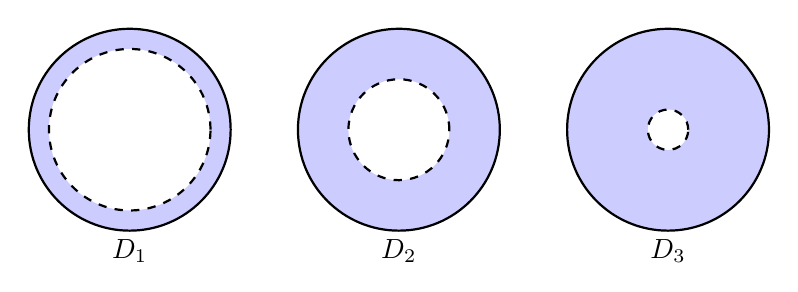
\begin{tikzpicture}
    \begin{axis}[
        axis lines = none,
        xmin=-2.5, xmax=10.5,
        ymin=-2, ymax=2,     
        width=15cm, height=5cm,
        axis equal image,
    ]
        % Gráfica para el disco 1
        \fill[blue!20] (0,0) circle [radius=1.5];
        \fill[white] (0,0) circle [radius=1.2];
        \draw[black, thick] (0,0) circle [radius=1.5];
        \draw[black, thick, dashed] (0,0) circle [radius=1.2];
        \node at (axis cs: 0, -1.80) {$D_1$};
        % Gráfica para el disco 2
        \fill[blue!20] (4,0) circle [radius=1.5];
        \fill[white] (4,0) circle [radius=0.75];
        \draw[black, thick] (4,0) circle [radius=1.5];
        \draw[black, thick, dashed] (4,0) circle [radius=0.75];
        \node at (axis cs: 4, -1.80) {$D_2$};
        % Gráfica para el disco 3
        \fill[blue!20] (8,0) circle [radius=1.5];
        \fill[white] (8,0) circle [radius=0.3];
        \draw[black, thick] (8,0) circle [radius=1.5];
        \draw[black, thick, dashed] (8,0) circle [radius=0.3];
        \node at (axis cs: 8, -1.80) {$D_3$};
    \end{axis}
\end{tikzpicture}
\caption{Representación de la familia $\{D_{\epsilon}\}_{\epsilon \in I}$}
\end{figure}

Luego, definir la unión de los conjuntos de $\{D_{\epsilon}\}_{\epsilon \in I}$ como:

$\bigcup_{\epsilon \in I} D_{\epsilon} = \{(x, y) \in \mathbb{R}^2 \mid x^2 + y^2 < 1^2\}$

\newpage
\textit{Ejemplo:}

Definir una familia $\{A_k\}_{k \in I}$ donde cada conjunto $A_k$ agrupe los primeros $k$ números pares positivos.

\textbf{Objetivo:} $A_1 = \{2\}, A_2 = \{2, 4\}, A_3 = \{2, 4, 6\}, \dots$

Dado el conjunto de índices $I = \mathbb{N} = \{1, 2, 3, ...\}$, la familia $\{A_K\}_{k \in I}$ se encuentra definida por la regla:

$A_k = \{2n \mid 1 \le n \le k, n \in \mathbb{N}\}$

Se podría desglosar:

$A_1 = \{2\}$

$A_2 = \{2, 4\}$

$A_3 = \{2, 4, 6\}$

$\dots$

Se define la unión de la familia como:

$\bigcup_{k \in I} A_k = \{2n \mid n \ge 1, n \in \mathbb{N}\} = \{2, 4, 6, \dots\}$

\textit{Ejemplo:}

Se necesita definir una familia de rectas $\{R_b\}_{b \in I}$, todas con pendiente 1, pero que cruzan el eje vertical ($Y$) en diferentes alturas $b$.

\textbf{Objetivo:} Las rectas deben pasar por el eje $Y$ en algún punto entre $-5$ y $5$ (incluyendo los extremos).

Dado el conjunto de índices $I = \{b \in \mathbb{R} \mid -5 \le b \le 5\}$, la familia de conjuntos $\{R_b\}_{b \in I}$ está definido por:

$R_b = \{(x, y) \in \mathbb{R} \mid y = x + b\}$

Como el intercepto $Y: b = y - x$, debe estar contenido en el intervalo $\left[-5, 5\right]$, es posible definir la unión de la familia como:

$\bigcup_{b \in I} R_b = \{(x, y) \in \mathbb{R} \mid -5 \le y - x \le 5\}$

\begin{figure}[H]
\centering
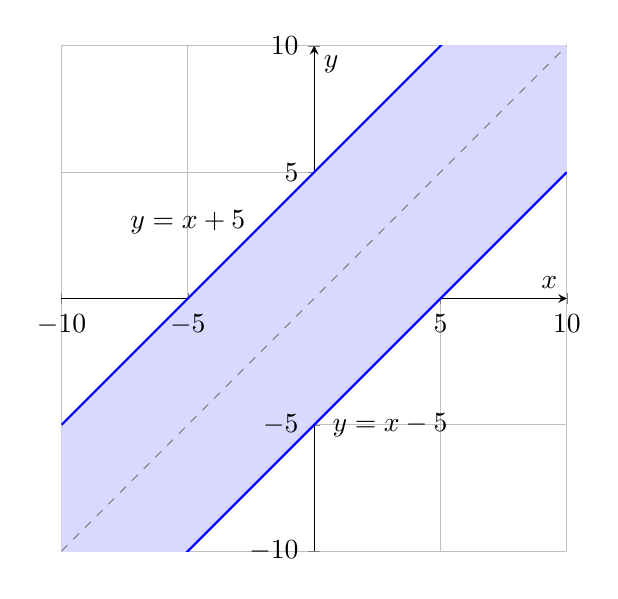
\begin{tikzpicture}
    \begin{axis}[
        axis lines = middle,
        xlabel = {$x$}, ylabel = {$y$},
        ymin=-10, ymax=10,
        xmin=-10, xmax=10,
        grid = major,
        width=8cm, height=8cm,
        axis equal image
    ]
        % Definición de las rectas con intercepto: Y = 5, Y = -5
        \addplot [name path=A, thick, blue, domain=-10:10] {x + 5};
        \addplot [name path=B, thick, blue, domain=-10:10] {x - 5};
        % Definición del área entre las rectas
        \addplot [blue!15] fill between [of=A and B];
        % Recta intermedia (b=0)
        \addplot [dashed, gray, domain=-10:10] {x};
        % Ecuación de las funciones
        \node at (axis cs: -5, 3) {$y = x + 5$};
        \node at (axis cs: 3, -5) {$y = x - 5$};
    \end{axis}
\end{tikzpicture}
\caption{Representación de la unión $\bigcup_{b \in I} R_b$.}
\end{figure}

\subsection{Intersección generalizada de familias}

Sea $\{A_i\}_{i \in I}$ una familia de conjuntos indexada por $I$. La intersección de la familia se define como el conjunto de todos los elementos que pertenecen a \textbf{cada uno} de los conjuntos $A_i$.

Se denota formalmente como:

\[ \bigcap_{i \in I} A_i = \{x \mid \forall i \in I, x \in A_i\} \]

\textit{Ejemplo:}

Considerar la misma familia de discos del ejercicio anterior:

$D_{\epsilon} = \{(x, y) \mid \epsilon^2 < x^2 + y^2 < 1^2\}$

Pero ahora, se debe hallar la \textbf{intersección} (si existe).

Para cualquier $(x, y) \in \mathbb{R}^2$, es cierto que $(x, y) \in \bigcap_{\epsilon \in I} D_{\epsilon}$, si se cumple con  $\epsilon^2 < x^2 + y^2 < 1^2, \forall \epsilon \in (0, 1)$.

Notar que \textbf{siempre} es posible encontrar un $\epsilon \in (0, 1)$, tal que $\epsilon^2 \ge x^2 + y^2$, con lo cual no se cumple la condición para estar en la intersección (específicamente $\epsilon^2 < x^2 + y^2$).

Por lo tanto, $\bigcap_{\epsilon \in I} D_{\epsilon} = \emptyset$

Por ejemplo, suponer el punto $(-0.3, 0.2) \implies r^2 = x^2 + y^2 = (-0.3)^2 + (0.2)^2 = 0.13$.

Basta con elegir un $\epsilon^2 \ge 0.13$ (por ejemplo, $\epsilon = 0.17$), para que el punto $(-0.3, 0.2)$ no se encuentre dentro del disco resultante:

\begin{figure}[H]
\centering
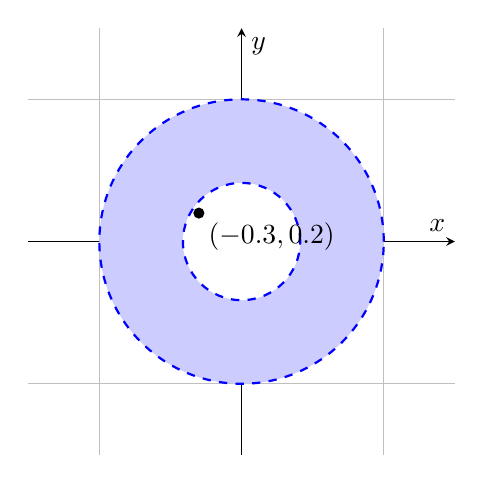
\begin{tikzpicture}
    \begin{axis}[
        axis lines = middle,
        xlabel = {$x$},
        ylabel = {$y$},
        ymin=-1.5, ymax=1.5,
        xmin=-1.5, xmax=1.5,
        grid = major,
        width=7cm, height=7cm,
        axis equal image,
        ticks = none
    ]
        % Anillo (el conjunto D_epsilon)
        \fill[blue!20] (0,0) circle [radius=1];
        \fill[white] (0,0) circle [radius=0.4123];
        % Bordes del disco
        \draw[thick, blue, dashed] (0,0) circle [radius=1];
        \draw[thick, blue, dashed] (0,0) circle [radius=0.4123];
        % Punto (-0.3, 0.2)
        \fill[black] (axis cs: -0.3, 0.2) circle (2pt) node[anchor=north west] {$(-0.3, 0.2)$};
    \end{axis}
\end{tikzpicture}
\caption{El punto $(-0.3, 0.2)$ excluido del disco perforado $D_{\epsilon}$ para $\epsilon^2 = 0.17$.}
\end{figure}

\textit{Ejemplo:}

Imaginar una familia de regiones en el plano que son triángulos rectángulos isósceles, cuyo vértice en el origen es fijo, pero sus catetos sobre los ejes se van haciendo cada vez más pequeños a medida que el índice $k$ aumenta su valor.

Dado el conjunto de índices $I = \{k \in \mathbb{R} \mid k > 0\}$, la familia $\{T_k\}_{k \in I}$ está definida por la regla de asignación:

$T_k = \{(x, y) \in \mathbb{R}^2 \mid x + y \le \frac{1}{k}, x \ge 0 \land y \ge 0\}$

Para cualquier punto $(x, y) \in \mathbb{R}^2$, es cierto que $(x, y) \in \bigcap_{k \in I} T_k$, si se cumple que $x + y \le \frac{1}{k}, \forall k > 0$.

Suponer, por ejemplo, un $k$ bastante pequeño: $k = 0.001 \implies \frac{1}{k} = \frac{1}{0.001} = 1000$.

En general, siempre se puede encontrar un punto $(x, y) \in \mathbb{R}^2$ tal que $x + y > \frac{1}{k}$ (lo cual rompe la condición para ser parte de la intersección). Dentro del contexto del ejemplo, se puede considerar el punto $(1000, 1) \in \mathbb{R}^2 \implies x + y = 1000 + 1 = 1001 > 1000 = \frac{1}{k}$.

El único punto que siempre cumple con $x + y \le \frac{1}{k}$ es $(0, 0) \in \mathbb{R}^2$, ya que $x + y = 0 + 0 = 0 \le \frac{1}{k}, \forall k > 0$.

Por lo tanto, $\bigcap_{k \in I} T_k = \{(0, 0)\}$.

\begin{figure}[H]
\centering
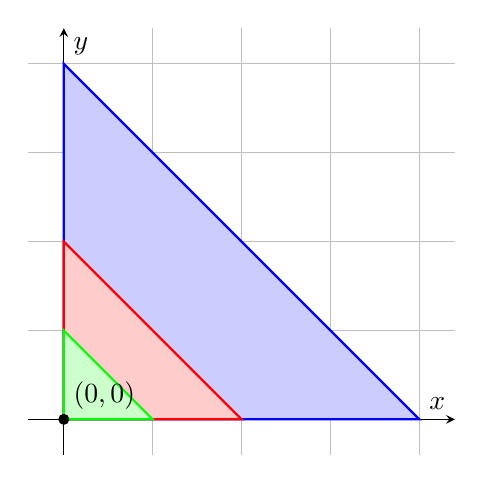
\begin{tikzpicture}
    \begin{axis}[
        axis lines = middle,
        xlabel = {$x$},
        ylabel = {$y$},
        ymin=-0.2, ymax=2.2,
        xmin=-0.2, xmax=2.2,
        grid = major,
        width=7cm, height=7cm,
        axis equal image,
        ticks = none
    ]
        % Triángulo 1 (k = 0.5, 1/k = 2)
        \fill[blue!20] (0,0) -- (2,0) -- (0,2) -- cycle;
        \draw[thick, blue] (0,0) -- (2,0) -- (0,2) -- cycle;
        % Triángulo 2 (k = 1, 1/k = 1)
        \fill[red!20] (0,0) -- (1,0) -- (0,1) -- cycle;
        \draw[thick, red] (0,0) -- (1,0) -- (0,1) -- cycle;
        % Triángulo 3 (k = 2, 1/k = 0.5)
        \fill[green!20] (0,0) -- (0.5,0) -- (0,0.5) -- cycle;
        \draw[thick, green] (0,0) -- (0.5,0) -- (0,0.5) -- cycle;
        % Punto origen
        \fill[black] (axis cs: 0, 0) circle (2pt) node[anchor=south west] {$(0,0)$};
    \end{axis}
\end{tikzpicture}
\caption{Gráfica de la familia de triángulos $\{T_k\}_{k \in I}$.}
\end{figure}

\textit{Ejemplo:}

Dado el conjunto de índices $I = \mathbb{N} = \{1, 2, 3, \dots\}$, la familia $\{A_n\}_{n \in \mathbb{N}}$ se encuentra definida por la regla:

$A_n = (0, \frac{1}{n})$

Determinar $\bigcap_{n \in \mathbb{N}} A_n$.

Es posible realizar el desglose de $A_n$ como:

$A_1 = (0, \frac{1}{1}) = (0, 1)$

$A_2 = (0, \frac{1}{2}) = (0, 0.5)$

$A_3 = (0, \frac{1}{3})$

$A_4 = (0, \frac{1}{4}) = (0, 0.25)$

$\dots$

$A_{1000} = (0, \frac{1}{1000}) = (0, 0.001)$

$\dots$

Observar dos cosas importantes:

\begin{itemize}
    \item Cada vez que $n$ aumenta su valor, $\frac{1}{n}$ se acerca cada vez más a cero.
    \item Para que un número $k \in \mathbb{R}^+$ pertenezca a $\bigcap_{n \in \mathbb{N}} A_n$, debe cumplirse con la condición que $k \in (0, \frac{1}{n}) \implies 0 < k < \frac{1}{n}, \forall n \in \mathbb{N}$.
\end{itemize}

Si se elige un valor $k \in \mathbb{R}^+$ bastante cercano al cero, por ejemplo $k = 0.000001$, \textbf{siempre} se puede encontrar un $n \in \mathbb{N}$ tal que $k > \frac{1}{n}$, lo cual rompería con la condición para ser parte de la intersección.

En el contexto del ejemplo, se supone que $k = \frac{1}{n} \implies n = \frac{1}{k} \implies n = \frac{1}{0.000001} = 1000000$.

Elegir un $n > 1000000$, por ejemplo $n = 1000001 \implies \frac{1}{n} = \frac{1}{1000001} \approx 0.0000009$. Lo anterior implica que $k = 0.000001 > \frac{1}{1000001} = \frac{1}{n}$.

Por lo tanto, se concluye que $\bigcap_{n \in \mathbb{N}} A_n = \emptyset$. 

\appendix

\section{Relaciones y clases de equivalencia (particiones)}

\subsection{Definición general}

Dados dos conjuntos no vacíos $A$ y $B$, una \textbf{relación binaria} $R$ de $A$ en $B$ se define formalmente como cualquier subconjunto del producto cartesiano $A \times B$.

\[R \subseteq A \times B = \{(a, b) \mid a \in A \land b \in B\}\]

Se dice que $a$ está relacionado con $b$, denotado por $aRb$, si y solo si $(a, b) \in R$.

\textit{Ejemplo:}

Sean los conjuntos $A = \{2, 3, 5\}$ y $B = \{10, 15, 20, 25\}$, definir la relación $R$ como:

$R = \{(a, b) \in A \times B \mid a \text{ divide a }b\}$

Primero se debe determinar $A \times B$:

Como $A$ y $B$ son conjuntos finitos, se tiene la siguiente cardinalidad:

$\left|A \times B \right| = \left|A\right| \times \left|B\right| \implies 3 \times 4 = 12$

$A \times B = \{(2, 10), (2, 15), (2, 20), (2, 25), (3, 10), (3, 15), (3, 20), (3, 25), (5, 10), (5, 15), (5, 20), (5, 25)\}$

Luego, seleccionar únicamente los pares que cumplen con la propiedad "$a \text{ divide a }b$":

$R = \{(2, 10), (2, 20), (3, 15), (5, 10), (5, 15), (5, 20), (5, 25)\}$

\textit{Ejemplo:}

Sean $A = \{1, 2, 3, 4, 5\}$ y $B = \{\left[1, 2\right], \left[3, 5\right]\}$, definir la relación $R$ de la siguiente manera:

$R = \{(a, I) \in A \times B \mid a \in I\}$

Nuevamente hallar el producto cartesiano $A \times B$, definiendo su cardinalidad: $\left|A \times B \right| = 5 \times 2 = 10$.

$\left|A \times B \right| = \{(1, \left[1, 2\right]), (1, \left[3, 5\right]), (2, \left[1, 2\right]), (2, \left[3, 5\right]), (3, \left[1, 2\right]), (3, \left[3, 5\right]), (4, \left[1, 2\right]), (4, \left[3, 5\right]), (5, \left[1, 2\right]), (5, \left[3, 5\right])\}$

Luego, elegir los pares de acuerdo a la propiedad de la relación $R$:

$R = \{(1, \left[1, 2\right]), (2, \left[1, 2\right]), (3, \left[3, 5\right]), (4, \left[3, 5\right], (5, \left[3, 5\right])\}$

\subsection{Relaciones en un conjunto $A$}

Cuando el dominio y codominio coinciden: $R \subseteq A \times A$, $R$ es una \textbf{relación en $A$}. Las propiedades fundamentales que rigen estas estructuras son:

\begin{itemize}
    \item \textbf{Reflexiva:} $\forall a \in A, (a, a) \in R$
    \item \textbf{Simétrica:} $\forall a,b \in A, (a, b) \in R \implies (b, a) \in R$
    \item \textbf{Antisimétrica:} $\forall a,b \in A, ((a, b) \in R \land (b, a) \in R) \implies a = b$
    \item \textbf{Transitiva:} $\forall a,b,c \in A, ((a, b) \in R \land (b, c) \in R) \implies (a, c) \in R$
\end{itemize}

\textit{Ejemplo:}

Sea $A = \mathbb{Z}$, definir la relación $R$ tal que $(a, b) \in R \iff a \equiv b \pmod 2$, es decir, tienen la misma paridad.

\underline{Nota:}

La expresión $a \equiv b \pmod n$ denota que $a$ y $b$ son \textbf{congruentes módulo $n$}. Esto significa que la diferencia $(a - b)$ es un múltiplo entero de $n$, o de forma equivalente, que $a$ y $b$ dejan el mismo residuo al ser divididos por una cantidad $n$.

\newpage
Determinar cuáles propiedades cumplen con la relación $R$:

\begin{itemize}
    \item \textbf{Reflexiva:} La relación $R$ es reflexiva ya que para todo $a \in A$, se cumple con $a \equiv a \pmod 2$. Por ejemplo,se sabe que $-7 \equiv -7 \pmod 2$, porque ambos números son iguales y su residuo es 1. \footnote{Según el Teorema de la División de Euclides, dados $a \in \mathbb{Z}$ y $m \in \mathbb{Z}^+$, existen únicos enteros $q$ (cociente) y $r$ (residuo) tales que $a = mq + r$, con $0 \leq r < m$.}
    \item \textbf{Simétrica:} La relación $R$ también es simétrica, ya que para cualesquiera $a, b \in A$ se cumple que $a \equiv b \pmod 2 \implies b \equiv a \pmod 2$. Suponer $14 \equiv 20 \pmod 2 \implies 20 \equiv 14 \pmod 2$.
    \item \textbf{Transitiva: } También es transitiva, ya que para cualesquiera $a, b, c \in A$, se tiene que $a \equiv b \pmod 2 \land b \equiv c \pmod 2 \implies a \equiv c \pmod 2$. Si se tiene que $-11 \equiv -13 \pmod 2 \land -13 \equiv -15 \pmod 2 \implies -11 \equiv -15 \pmod 2$.
    \item \textbf{Antisimétrica: } No, la relación $R$ no es antisimétrica. Por contraejemplo, se tiene $6 \equiv 4 \pmod 2 \land 4 \equiv 6 \pmod 2$, no implica que $4$ y $6$ sean iguales.
\end{itemize}

\textit{Ejemplo:}

Sea $A = \{1, 2, 3, 4 , 6\}$, definir la relación $R = \{(a, b) \mid a|b\}$.

La propiedad $a | b$ implica que existe un $k \in \mathbb{Z}$ tal que $b = ak \implies k = \frac{b}{a}$. 

\begin{table}[h!]
\centering
\begin{tabular}{r|ccccc}
$a \mid b$ & \textbf{1} & \textbf{2} & \textbf{3} & \textbf{4} & \textbf{6} \\ \hline
\textbf{1} & \checkmark & \checkmark & \checkmark & \checkmark & \checkmark \\
\textbf{2} & & \checkmark & & \checkmark & \checkmark \\
\textbf{3} & & & \checkmark & & \checkmark \\
\textbf{4} & & & & \checkmark & \\
\textbf{6} & & & & & \checkmark \\
\end{tabular}
\caption{Relación de divisibilidad en $A$.}
\end{table}

$R = \{(1, 1), (1, 2), (1, 3), (1, 4), (1, 6), (2, 2), (2, 4), (2, 6), (3, 3), (3, 6), (4, 4), (6, 6)\}$

Revisar que propiedad cumple la relación $R$:

\begin{itemize}
    \item \textbf{Reflexiva:} Si, la relación $R$ es reflexiva ya que para todo $a \in A$ se cumple que $(a, a) \in R$.
    \item \textbf{Simétrica:} Por contraejemplo, se tiene que el elemento $(1, 2) \in R$, pero $(2, 1) \not \in R$. Por lo tanto, la relación $R$ no es simétrica.
    \item \textbf{Transitiva:} La relación $R$ también es transitiva: Si $a, b, c \in A$, se cumple que $(a, b) \in R \land (b, c) \in R \implies (a, c) \in R$.
    \item \textbf{Antisimétrica:} Si, la relación $R$ es antisimétrica, es decir, para cualesquiera $a, b \in A$ se cumple con $(a, b) \in R \land (b, a) \in R \implies a = b$.
\end{itemize}

A continuación la \textbf{demostración} para la propiedad (antisimetría):

Como $(a, b) \in R \implies b = ak_1$, para $k_1 \in \mathbb{Z}^+$

Además, como $(b, a) \in R \implies a = bk_2$, para $k_2 \in \mathbb{Z}^+$

Sustituir $a$ en la primera ecuación:

$b = ak_1 \implies b = (bk_2)k_1 \implies b = b(k_1k_2)$

Lo anterior implica necesariamente que $k_1k_2 = 1 \implies k_1 = 1 \land k_2 = 1$

Por lo tanto:

$b = ak_1 \implies b = a(1) = a$

$a = bk_2 \implies a = b(1) = b$

$\qed$

\subsection{Relaciones de equivalencia}

Una relación de equivalencia es una forma de agrupar elementos de un conjunto que "se comportan igual" bajo cierto criterio. Para que una relación $\sim$ en un conjunto $A$ sea de equivalencia debe cumplir con ser:

\begin{itemize}
    \item \textbf{Reflexiva:} Todo elemento está relacionado consigo mismo ($a \sim a$).
    \item \textbf{Simétrica:} Si $a$ está relacionado con $b$, entonces $b$ está relacionado con $a$ ($a \sim b \implies b \sim a$).
    \item \textbf{Transitiva:} Si $a$ está relacionado con $b$ y $b$ con $c$, entonces $a$ está relacionado con $c$ ($a \sim b \land b \sim c \implies a \sim c$).
\end{itemize}

\subsection{Clase de equivalencia}

Cuando se tiene una relación de equivalencia, es posible formar "grupos". La \textbf{clase de equivalencia} de un elemento $a$, denotado como $\left[a\right]$, es el conjunto de todos los elementos de $A$ que están relacionados con $a$.

\subsection{Particiones}

Una \textbf{partición} de un conjunto $A$ es una colección de subconjuntos no vacíos de $A$, tales que:

\begin{itemize}
    \item \textbf{Son disjuntos:} Si se toman dos subconjuntos diferentes, su intersección es vacía (no comparten elementos).
    \item \textbf{Su unión es el total:} Si se juntan todos los subconjuntos, se recupera el conjunto $A$ completo.
\end{itemize}

\textbf{Teorema fundamental:} Toda relación de equivalencia en $A$ crea una partición de $A$ (donde las clases de equivalencia son los subconjuntos). Y toda partición de $A$ define una relación de equivalencia.

\textit{Ejemplo:}

Se tiene el conjunto de números enteros $\mathbb{Z}$.

Definir la relación $\sim$ tal que:

$a \sim b$ si y solo si $a \text{ y } b$ tienen el mismo residuo al dividirlos entre 3.

\textbf{a) Relación de equivalencia:}

Para que sea relación de equivalencia, debe cumplir tres propiedades:

\begin{itemize}
    \item \textbf{Reflexiva:} Cualquier entero $a$ tiene el mismo resto que sí mismo al dividirlo por 3. Por ejemplo, 4 y 4 tienen el mismo resto 1.
    \item \textbf{Simétrica:} Si 7 tiene el mismo resto que 4, entonces 4 tiene el mismo resto que 7 (el resto es 1).
    \item \textbf{Transitiva:} Si 10 tiene el mismo resto que 7 (el resto es 1), y 7 tiene el mismo resto que 4, entonces, 10 tiene el mismo resto que 4.
\end{itemize}

\textbf{b) Clase de equivalencia:}

Como esta relación es de equivalencia, se puede agrupar a todos los números en grupos según su resto. En este caso, solo hay 3 posibles restos al dividir por 3: 0, 1 y 2.

\begin{itemize}
    \item $\left[0\right] = \{\dots, -9, -6, -3, 0, 3, 6, 9, \dots\}$
    \item $\left[1\right] = \{\dots, -7, -4, -1, 1, 4, 7, \dots\}$
    \item $\left[2\right] = \{\dots, -8, -5, -2, 2, 5, 8, \dots \}$
\end{itemize}

\textbf{c) Particiones}:

Dadas las clases de equivalencia, se puede observar que:

\begin{itemize}
    \item $\left[0\right] \cap \left[1\right] \cap \left[2\right] = \emptyset$
    \item $\left[0\right] \cup \left[1\right] \cup \left[2\right] = \mathbb{Z}$
\end{itemize}

\textit{Ejemplo:}

Suponer que actualmente se está diseñando un sistema de base de datos. Considerar el conjunto $S$ de todas las palabras (cadenas de texto) que no están vacías (en Español). 

Definir la relación $\sim$ así:

$R:$ Dos palabras $s_1 \text{ y } s_2$ están relacionadas ($s_1 \sim s_2$) si y solo si comienzan con la misma letra.

\textbf{a) Relación de equivalencia:}

Para que la relación $R$ sea una relación de equivalencia debe cumplir con las propiedades:

\begin{itemize}
    \item \textbf{Reflexiva:} Cualquier palabra $p$ comienza con la misma letra que sí misma. Por ejemplo, "perro" y "perro" comienzan con la misma letra "p".
    \item \textbf{Simétrica:} Si la palabra "papá" comienza con la misma letra "p" que la palabra "perro", entonces "perro" comienza con la misma letra que "papá".
    \item \textbf{Transitiva:} Si la palabra "pala" comienza con la misma letra "p" que la palabra "papá", y "papá" comienza con la misma letra que "perro", entonces "pala" comienza con la misma letra que "perro".
\end{itemize}

Entonces, se puede concluir que $R$ es una \textbf{relación de equivalencia}.

\textbf{b) Clase de equivalencia:}

Como $R$ es una relación de equivalencia, se puede formar subconjuntos del conjunto de todas las palabras en Español, basados en su primera letra:

$\left[a\right] = \{\text{árbol, alameda, araña, }\dots\}$

$\left[b\right] = \{\text{barco, balón, ballena, }\dots\}$

$\left[c\right] = \{\text{casa, cedro, comida, }\dots\}$

$\dots$

$\left[z\right] = \{\text{zanahoria, zapato, zanja, }\dots\}$

\textbf{c) Particiones:}

Dadas las clases de equivalencia, notar que:

\begin{itemize}
    \item Son disjuntas par a par, por ejemplo: $\left[a\right] \cap \left[b\right] = \emptyset$
    \item $\left[a\right] \cup \left[b\right] \cup ... \cup \left[z\right] = \text{ todas las palabras en Español}$
\end{itemize}

\textit{Ejemplo:}

Considerar el conjunto de todos los puntos del plano cartesiano $\mathbb{R}^2$. 

Definir la relación $\sim$ como: 

$R: (x_1, y_1) \sim (x_2, y_2)$ si y solo si $y_1 = y_2$

\textbf{a) Relación de equivalencia:}

La relación $R$ es una relación de equivalencia, si cumple con las siguientes propiedades:

\begin{itemize}
    \item \textbf{Reflexiva:} Cualquier punto $(x, y) \in \mathbb{R}^2$, tendrá la misma coordenada $y$ que si mismo. Por ejemplo, los puntos $(4, -7)$ y $(4, -7)$ tienen la misma coordenada en $y = -7$.
    \item \textbf{Simétrica:} Si el punto $(4, -7)$ tiene la misma coordenada $y = -7$ que el punto $(-2, -7)$, entonces $(-2, -7)$ tiene la misma coordenada $y$ que el punto $(4, -7)$.
    \item \textbf{Transitiva:} Si el punto $(11, -7)$ tiene la misma coordenada $y = -7$ que el punto $(-2, -7)$, y $(-2, -7)$ tiene la misma coordenada $y$ que el punto $(4, -7)$, entonces $(11, -7)$ tiene la misma coordenada $y$ que el punto $(4, -7)$.
\end{itemize}

Por lo tanto, la relación $R$ es una relación de equivalencia.

\textbf{b) Clases de equivalencia:}

Como $R$ es una relación de equivalencia, es posible formar subconjuntos de $\mathbb{R}^2$, basados en la relación $y_1 = y_2$:

$C_k = \{(x, y) \in \mathbb{R}^2 \mid y = k\}$

Geométricamente, cada subconjunto representa una \textbf{recta horizontal} en el plano cartesiano $XY$.

\textbf{c) Particiones:}

Dadas las clases de equivalencia, se debe observar que:

\begin{itemize}
    \item Son disjuntas par por par, por ejemplo: $\left[(x, 2)\right] \cap \left[(x, -2)\right] = \emptyset$ (de hecho, estas rectas son paralelas).
    \item $\bigcup_{k \in \mathbb{R}} C_k = \mathbb{R}^2$
\end{itemize}

\subsection{Relaciones de orden}

Mientras las relaciones de equivalencia sirven para \textbf{agrupar}, las relaciones de orden sirven para \textbf{organizar}.

Para que una relación sea de orden (específicamente de \textbf{orden parcial}), debe cumplir con tres propiedades obligatorias:

\begin{itemize}
    \item \textbf{Reflexiva:} Todo elemento se compara consigo mismo.
    \item \textbf{Antisimétrica:} Si $a$ va antes que $b$ y $b$ va antes que $a$, entonces tienen que ser el mismo.
    \item \textbf{Transitiva:} Si $a$ es menor que $b$, y $b$ es menor que $c$, entonces $a$ es menor que $c$.
\end{itemize}

\textit{Ejemplo:}

Comprobar si el conjunto de los números reales $\mathbb{R}$ es una relación de orden.

Entonces, el conjunto $\mathbb{R}$ es una relación de orden si cumple con ser:

\begin{itemize}
    \item \textbf{Reflexiva:} Si, el conjunto de los números reales es reflexiva, porque para cualquier $a \in \mathbb{R}$, la proposición $a \le a$ es verdadera (ya que $a = a$ es cierto).
    \item \textbf{Antisimétrica:} También es antisimétrica, ya que para cualesquiera $a, b \in \mathbb{R}$ se tiene que: Si $a \le b \land b \le a \implies a = b$. Por ejemplo, suponer $x \in \mathbb{R}$, si $5 \le x$ y $x \le 5 \implies x = 5$.
    \item \textbf{Transitiva:} Si, $\mathbb{R}$ es transitiva, ya que para cualesquiera $x, y, z \in \mathbb{R}$ se cumple que: Si $x \le y$ y $y \le z \implies x \le z$. Por ejemplo, suponer $-10, -5, -1 \in \mathbb{R}$, se sabe que $-10 \le -5$ y $-5 \le -1 \implies -10 \le -1$. 
\end{itemize}

Por lo tanto, el conjunto $\mathbb{R}$ es una relación de orden.

\textit{Ejemplo:}

Sea el conjunto de puntos en el plano $A = \mathbb{R}^2$.

Definir la relación $\preceq$ entre dos puntos $(x_1, y_1)$ y $(x_2, y_2)$ como:

$(x_1, y_1) \preceq (x_2, y_2) \iff x_1 \le x_2 \land y_1 \le y_2$

Comprobar que la relación $\preceq$ es una relación de orden.

Nuevamente, se necesita demostrar que las siguientes propiedades se cumplen para la relación:

\begin{itemize}
    \item \textbf{Reflexiva:} La relación es reflexiva, porque para cualquier $(x, y) \in \mathbb{R}^2$, la proposición $(x, y) \preceq (x, y)$ es verdadera (es cierto que $(x, y) = (x, y)$). 
    \item \textbf{Antisimétrica:} Si, la relación también es antisimétrica, ya que cumple con: Si $(x_1, y_1) \preceq (x_2, y_2)$ y $(x_2, y_2) \preceq (x_1, y_1) \implies (x_1, y_1) = (x_2, y_2)$. Por ejemplo, suponer que $(x, y) \in \mathbb{R}^2$ tal que $(1, 3) \preceq (x, y)$ y $(x, y) \preceq (1, 3)$, implica necesariamente que son el mismo punto: $(x, y) = (1, 3)$.
    \item \textbf{Transitiva:} La relación también es transitiva, ya que para cualesquiera $(x_1, y_1), (x_2, y_2), (x_3, y_3) \in \mathbb{R}^2$ se cumple que: Si $(x_1, y_1) \preceq (x_2, y_2) \land (x_2, y_2) \preceq (x_3, y_3) \implies (x_1, y_1) \preceq (x_3, y_3).$ Por ejemplo, si se tienen los puntos $A = (0, 0), B= (1, 1), C = (2, 2) \in \mathbb{R}^2$, se puede notar en el plano cartesiano que $A$ está abajo y a la izquierda de $B$, entonces $A \preceq B$. También se observa que $B$ está abajo y a la izquierda de $C$, por lo tanto $B \preceq C$. Finalmente, el punto $A$ está abajo y a la izquierda de $C$, es decir, $A \preceq C$, con lo cual se cumple la propiedad transitiva. 
\end{itemize}

\begin{figure}[h!]
\centering
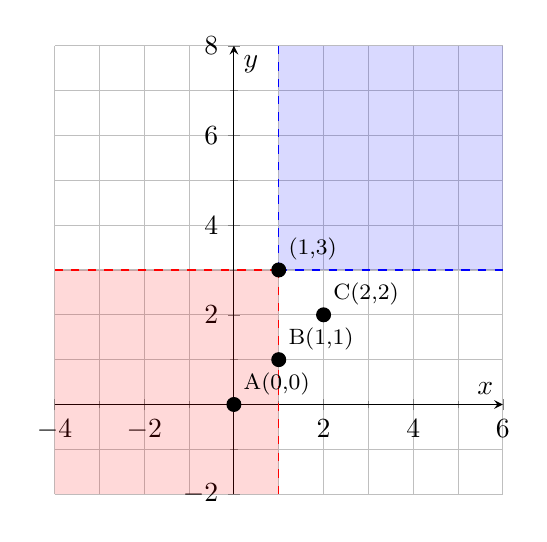
\begin{tikzpicture}
\begin{axis}[
    axis lines = middle,   
    xmin=-4, xmax=6,        
    ymin=-2, ymax=8,        
    xlabel=$x$, ylabel=$y$, 
    grid = both,            
    minor tick num=1,       
    unit vector ratio=1 1, 
]
\addplot[fill=blue, opacity=0.15, draw=none] coordinates {(1,3) (6,3) (6,8) (1,8) (1,3)}; 
\addplot[fill=red, opacity=0.15, draw=none] coordinates {(1,3) (-4,3) (-4,-2) (1,-2) (1,3)}; 
\draw[blue, dashed] (1,3) -- (6,3); \draw[blue, dashed] (1,3) -- (1,8);
\draw[red, dashed] (1,3) -- (-4,3); \draw[red, dashed] (1,3) -- (1,-2);
\addplot[
    only marks,             
    mark=*,                 
    mark size=2.5pt,          
    mark options={fill=black}, 
    nodes near coords,      
    every node near coord/.append style={
        anchor=south west,  
        font=\footnotesize         
    },
    point meta=explicit symbolic,
] coordinates {
    (0,0) [A(0,0)] 
    (1,1) [B(1,1)] 
    (2,2) [C(2,2)]
    (1,3) [(1,3)]
};
\end{axis}
\end{tikzpicture}
\caption{Visualización de antisimetría y transitividad.}
\end{figure}

\section{La infinitud de Dedekind}

Un conjunto es infinito si puede ser puesto en \textbf{biyección} con un subconjunto propio de sí mismo.

\textit{Ejemplo:}

Demostrar que el conjunto $P$ definido como: $P = \{2n \mid n \in \mathbb{N}\} = \{2, 4, 6, \dots\}$

Es un \textbf{conjunto infinito} en base a la infinitud de Dedekind.

Definir un subconjunto propio de conjunto $P$, por ejemplo el conjunto de los múltiplos de 10:

$D = \{10n \mid n \in \mathbb{N}\} = \{10, 20, 30, \dots\} \subsetneq P$

Generar la función $f: P \to D$, definida por $f(p) = 5p$

a) Demostrar que la función $f$ es inyectiva:

$\forall a, b \in P$ se tiene que $f(a) = f(b) \implies 5a = 5b \implies 5a - 5b = 0 \implies 5(a - b) = 0$

Implica necesariamente que $a - b = 0 \implies a = b$

Entonces, la función $f$ es inyectiva.

b) Demostrar que la función $f$ es sobreyectiva:

PD: $\forall d \in \text{Codom($f$)} = D, \exists p \in \text{Dom($f$)} = P$, tal que $f(p) = d$.

\underline{Hipótesis:}

Sea $d \in \text{Codom($f$)}$ arbitrario.

Demostrar que existe $p \in \text{Dom($f$)}$, tal que $f(p) = d$.

Se sabe que $\displaystyle 5p = d \implies p = \frac{d}{5}$

Como $d \in \text{Codom($f$)}$ y $\text{Codom($f$)} = D$, implica que $d = 2 \times 5 \times k$, con $k \in \mathbb{N}$.

Se tiene que $\displaystyle p = \frac{2 \times 5 \times k}{5} = 2k$, significa que $p$ es un número par positivo, por lo tanto, $p \in P = \text{Dom($f$)}$.

Evaluar $p$ en la función $f$:

$\displaystyle f(p) = 5\Big(\frac{d}{5}\Big) = d$

Entonces, la función $f$ es sobreyectiva.

Por (a) y (b) se puede concluir que $f$ es \textbf{biyectiva}.

Por infinitud de Dedekind, se sabe que el conjunto $P$ es un \textbf{conjunto infinito}.

$\qed$

\textit{Ejemplo:}

En base a la infinitud de Dedekind, demostrar que el conjunto de los números enteros $\mathbb{Z}$ es infinito.

Definir un subconjunto de $\mathbb{Z}$ como sigue:

$\mathbb{Z}^- = \{z \in \mathbb{Z} \mid z < 0\} \subsetneq \mathbb{Z}$

Luego, definir la función $f: \mathbb{Z} \to \mathbb{Z}^-$, dada por:

$
f(z) = 
\begin{cases}
    -2z - 1 \text{ si } z \ge 0 \\
    2z \text{ si } z < 0
\end{cases}
$

a) Demostrar que $f$ es \textbf{inyectiva}:

\textbf{Caso No. 1:} 

Para cualesquiera $a, b \in \mathbb{Z}$, con $a, b \ge 0$, se cumple que:

$f(a) = f(b) \implies -2a - 1 = -2b - 1 \implies -2a = -2b \implies -2a + 2b = 0 \implies -2(a - b) = 0$

Implica inevitablemente que $a - b = 0 \implies a = b$

Entonces, la función $f$ es inyectiva cuando $a, b$ son enteros positivos o cero.

\textbf{Caso No. 2:}

Para cualesquiera $a, b \in \mathbb{Z}$, con $a, b < 0$, se cumple que:

$f(a) = f(b) \implies 2a = 2b \implies 2a - 2b = 0 \implies 2(a - b) = 0$

Implica que $a - b = 0 \implies a = b$

Nuevamente, la función $f$ es inyectiva cuando $a, b$ son enteros negativos.

\textbf{Caso No. 3:}

Para cualesquiera $a, b \in \mathbb{Z}$, con $a \ge 0 \text{ y } b < 0$ (o viceversa), se tiene que:

Por la definición de la función $f$, se sabe que $f(a)$ será un número negativo impar, mientras que $f(b)$ generará un número negativo par, implica que siempre se tendrá $f(a) \neq f(b)$.

Entonces, la función $f$ es inyectiva cuando los valores tienen signos distintos.

Por los tres casos anteriores, se concluye que la función $f$ es \textbf{inyectiva}.

b) Demostrar que $f$ es \textbf{sobreyectiva}:

\textbf{Caso No. 1:}

PD: $\forall b \in \text{Codom($f$)} = \mathbb{Z}^-$ con $b$ impar, $\exists a \in \text{Dom($f$)} = \mathbb{Z}$, tal que $f(a) = b$.

\newpage
\underline{Hipótesis:}

Sea $b \in \text{Codom($f$)}$ arbitrario, con la única condición que $b$ sea impar.

Demostrar que $a \in \text{Dom($f$)}$, tal que $f(a) = b$.

Como $b \in \text{Codom($f$)} = \mathbb{Z}^- \ \land \ b \text{ es impar, significa que $b$ es un número impar negativo}.$ 

Es posible expresar $b = -2k - 1$, con $k \in \mathbb{N} \cup \{0\}$.

Debido a que $b$ es un impar negativo, aplica la primera parte de $f$:

$\displaystyle -2a - 1 = b \implies a = -\frac{b + 1}{2} \implies a = -\frac{(-2k - 1) + 1}{2} \implies a = -\frac{-2k}{2} = k$.

Por consiguiente, $a \in \mathbb{N} \cup \{0\}$ y como $\mathbb{N} \cup \{0\} \subseteq \mathbb{Z} \implies a \in \mathbb{Z}$.

Evaluar $a$ en la función $f$:

$\displaystyle f(a) = -2\Big(-\frac{b + 1}{2}\Big) - 1 = b + 1 - 1 = b$

Entonces, la función $f$ es sobreyectiva.

\textbf{Caso No. 2:}

PD: $\forall b \in \text{Codom($f$)} = \mathbb{Z}^- \text{ con $b$ par }, \exists a \in \text{Dom($f$)} = \mathbb{Z}$, tal que $f(a) = b$.

\underline{Hipótesis:}

Dado $b \in \text{Codom(f)}$ arbitrario, con la única condición que $b$ sea par. 
  
Demostrar que $a \in \text{Dom($f$)}$, tal que $f(a) = b$.

Como $b \in \text{Codom($f$)} = \mathbb{Z}^- \ \land \ b \text{ es un número par, implica que $b$ es un número par negativo}.$

Se puede expresar $b = -2k$, con $k \in \mathbb{N}$.

Como $b$ es un número par negativo, aplica la segunda parte de la función $f$, es decir:

$\displaystyle 2a = b \implies a = \frac{b}{2} \implies a = \frac{-2k}{2} = -k \in \mathbb{Z}^-$

Entonces, se tiene $a \in \mathbb{Z}^-$, como $\mathbb{Z}^- \subseteq \mathbb{Z} \implies a \in \mathbb{Z}$.

Se evalúa $a$ en la función $f$:

$\displaystyle f(a) = 2\Big(\frac{b}{2}\Big) = b$

Por lo tanto, la función $f$ es sobreyectiva. 

Por los dos casos anteriores, se puede concluir que $f$ es una función \textbf{sobreyectiva}.

Por lo tanto, la función $f$ es \textbf{biyectiva}.

Se ha demostrado, mediante infinitud de Dedekind, que el conjunto $\mathbb{Z}$ es un conjunto infinito.

$\qed$

\section{Leyes de De Morgan}

Las leyes de De Morgan son dos reglas fundamentales en la lógica y en la teoría de conjuntos que describen la relación entre las operaciones de unión e intersección en conjuntos, así como operaciones de negación en lógica:

\begin{itemize}
    \item $\sim(A \cup B) = \sim A \cap \sim B$
    \item $\sim(A \cap B) = \sim A \cup \sim B$
\end{itemize}

\subsection{Demostraciones}

1. $\sim(A \cup B) = \sim A \cap \sim B$

Demostrar mediante \textbf{doble contención:}

a) $\sim(A \cup B) \subseteq \sim A \cap \sim B$

\underline{Hipótesis:}

$x \in \sim(A \cup B)$

Es posible expresar la hipótesis como $x \not \in (A \cup B)$

Por definición de \textbf{unión} y \textbf{no pertenencia}, se tiene que $x$ no está en el conjunto $A$, o en el conjunto $B$, o en ambos conjuntos (la intersección), por lo tanto: 

$x \not \in A \land x \not \in B \implies x \in \sim A \land x \in \sim B$

Por definición de \textbf{intersección} se tiene:

$x \in \sim A \cap \sim B$

b) $\sim A \cap \sim B \subseteq \sim(A \cup B)$

\underline{Hipótesis:}

$x \in \sim A \cap \sim B$

Se tiene que $x \in \sim A \land x \in \sim B \implies x \not \in A \land x \not \in B$

Lo anterior implica que $x$ no está en el conjunto $A$ y tampoco está en el conjunto $B$ (lo que también incluye su intersección), por lo tanto: $x \not \in (A \cup B) \implies x \in \sim (A \cup B) \qed$

\begin{figure}[H]
    \centering
    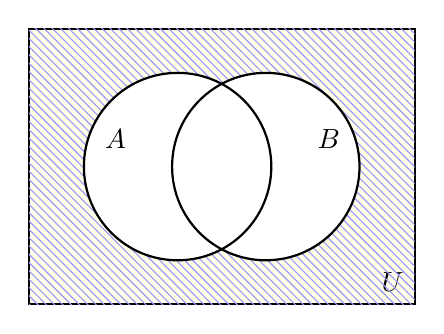
\begin{tikzpicture}[scale=0.7]
        \colorlet{fondoU}{yellow!10}
        \fill[fondoU] (-3.5,-2.5) rectangle (3.5,2.5);
        \draw[thick] (-3.5,-2.5) rectangle (3.5,2.5);
        \node[fill=fondoU, thin, inner sep=2pt] at (3.1,-2.1) {$U$};
        \begin{scope}
            \clip (-3.5,-2.5) rectangle (3.5,2.5);
            \pattern[pattern=north west lines, pattern color=blue!40] (-3.5,-2.5) rectangle (3.5,2.5);
            \fill[white] (-0.8,0) circle (1.7);
            \fill[white] (0.8,0) circle (1.7);
        \end{scope}
        \draw[thick] (-0.8,0) circle (1.7) node[left=15pt, yshift=10pt] {$A$};
        \draw[thick] (0.8,0) circle (1.7) node[right=15pt, yshift=10pt] {$B$};
    \end{tikzpicture}
    \caption{Visualización de la propiedad $\sim(A \cup B) = \sim A \cap \sim B$.}
\end{figure}

2. $\sim(A \cap B) = \sim A \cup \sim B$

Nuevamente, se necesita demostrar por \textbf{doble contención:}

a) $\sim (A \cap B) \subseteq \sim A \cup \sim B$

\underline{Hipótesis:}

$x \in \sim (A \cap B)$

Plantear la hipótesis como $x \not \in (A \cap B)$

Esto significa que $x$ no pertenece a la intersección de los conjuntos $A$ y $B$, implica que $x$ no está en el conjunto $A$, o no está en el conjunto $B$. Por lo tanto, se tiene:

$x \not \in A \lor x \not \in B \implies x \in \sim A \lor x \in \sim B$

Por definición de \textbf{unión} se tiene que:

$x \in \sim A \cup \sim B$

b) $\sim A \cup \sim B \subseteq \sim(A \cap B)$

\underline{Hipótesis:}

$x \in \sim A \cup \sim B$

Por definición de \textbf{unión} se tiene $x \in \sim A \lor x \in \sim B \implies x \not \in A \lor x \not \in B$

Para que $x$ esté en $(A \cap B)$ necesariamente debe pertenecer al conjunto $A$ y a $B$ al mismo tiempo, por lo tanto, $x \not \in A \lor x \not \in B$ implica que: 

$x \not \in (A \cap B) \implies x \in \sim (A \cap B)$

$\qed$

\begin{figure}[H]
    \centering
    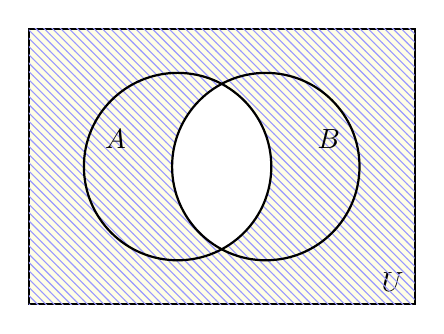
\begin{tikzpicture}[scale=0.7]
        \colorlet{fondoU}{yellow!10}
        \fill[fondoU] (-3.5,-2.5) rectangle (3.5,2.5);
        \draw[thick] (-3.5,-2.5) rectangle (3.5,2.5);
        \node[fill=fondoU, inner sep=2pt] at (3.1,-2.1) {$U$};
        \begin{scope}
            \pattern[pattern=north west lines, pattern color=blue!40] (-3.5,-2.5) rectangle (3.5,2.5);
            \begin{scope}
                \clip (-0.8,0) circle (1.7);
                \fill[white] (0.8,0) circle (1.7);
            \end{scope}
        \end{scope}
        \draw[thick] (-0.8,0) circle (1.7) node[left=15pt, yshift=10pt] {$A$};
        \draw[thick] (0.8,0) circle (1.7) node[right=15pt, yshift=10pt] {$B$};
    \end{tikzpicture}
    \caption{Visualización de la propiedad $\sim(A \cap B) = \sim A \cup \sim B$.}
\end{figure}

\section{Ejercicios aplicados}

\subsection{Sobre conjuntos y operaciones (estructura de datos)}

\textbf{1. Modelado de bases de datos NoSQL:} Suponer que se representan las etiquetas (tags) de tres artículos de un blog como conjuntos $A, B \text{ y } C$. Se necesita expresar mediante operaciones de conjuntos cómo se obtendrían los artículos que tienen etiquetas en común entre $A \text{ y } B$ pero que no están presentes en $C$.

\textbf{Respuesta: } $(A \cap B) - C$

\textbf{2. Optimización de consultas:} En un motor de búsqueda, el conjunto $U$ son todas las páginas web. Si $P$ es el conjunto de páginas que contienen la palabra "Python" y $J$ las que contienen "Java", se debe utilizar las Leyes de De Morgan para expresar de una forma alternativa el conjunto de páginas que no contienen ninguna de las dos palabras.

\textbf{Respuesta: } $\sim(P \cup J) = \sim P \cap \sim J$

\underline{Nota:}

En términos de motores de búsqueda, implica que se pasa de un "NOT (Python OR Java)" a un "NOT Python AND NOT Java", lo cual suele ser más eficiente para procesar índices invertidos. 

\subsection{Sobre relaciones y funciones (algoritmos)}

\textbf{3. Funciones Hash:} Sea $S$ el conjunto de todos los posibles nombres de usuario y $K = \{0, 1, 2, 3, \dots, 999\}$ el conjunto de índices de una tabla. Si se define una función $h: S \to K$, explicar qué propiedad de las funciones se pierde cuando ocurre una "colisión" (dos usuarios distintos mapeados al mismo índice).

\textbf{Respuesta:}

Suponer el escenario en el cual se asigna un mismo índice a distintos usuarios:

Usuario 1: Edwin Lee $\to$ 18

Usuario 2: Noemi Hernández $\to$ 18

Para que la función $h$ sea \textbf{inyectiva} debería cumplir con:

$h(\text{Usuario 1}) = h(\text{Usuario 2}) \implies \text{Usuario 1} = \text{Usuario 2}$

Sin embargo, se sabe que: 

Edwin Lee $\neq$ Noemi Hernández

Por lo tanto, la función $h$ no puede ser inyectiva.

\textbf{4. Relaciones en grafos:} Un grafo dirigido se puede definir como un conjunto de vértices $V$ y una relación $R$ sobre $V \times V$. Si la relación $R$ es transitiva, ¿qué significa esto en términos de "caminos" entre los nodos del grafo?

Definir un conjunto de vértices $V = \{A, B, C\}$

Luego, se deb determinar la relación:

$R = V \times V = \{(A, A), (A, B), (A, C), (B, A), (B, B), (B, C), (C, A), (C, B), (C, C)\}$

La relación $R$ es \textbf{transitiva} ya que cumple con: Para cualquier $a, b, c \in V$ se cumple que $(a, b) \in R \land (b, c) \in R \implies (a, c) \in R$. Por ejemplo, para $A, B, C \in V$, se tiene que $(A, B) \in R \land (B, C) \in R \implies (A, C) \in R$.

Esto quiere decir que si existe un camino del nodo $A$ al $B$, y una ruta del $B$ al $C$, la transitividad implica necesariamente que existe un camino directo (un atajo) del nodo $A$ al $C$.

\begin{figure}[h!]
\centering
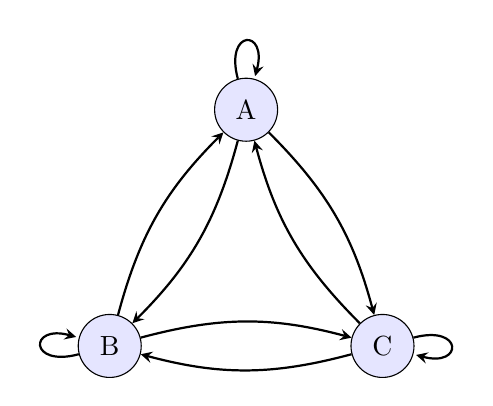
\begin{tikzpicture}[
    >={stealth},
    node distance=3cm,
    every node/.style={circle, draw, fill=blue!10, minimum size=8mm}
]
\node (A) at (90:2) {A};
\node (B) at (210:2) {B};
\node (C) at (330:2) {C};
\path[->, thick] 
    (A) edge [loop above] (A)
    (B) edge [loop left] (B)
    (C) edge [loop right] (C)
    (A) edge [bend left=15] (B)
    (B) edge [bend left=15] (A)
    (B) edge [bend left=15] (C)
    (C) edge [bend left=15] (B)
    (A) edge [bend left=15] (C)
    (C) edge [bend left=15] (A);
\end{tikzpicture}
\caption{Representación del grafo completo $V \times V$. La transitividad implica que cualquier secuencia de saltos tiene una conexión directa.}
\end{figure}

\subsection{Sobre inducción matemática (análisis de algoritmos)}

\textbf{5. Complejidad de bucles:} Utilizando el principio de inducción, se demostrará que la suma de los primeros $n$ números impares (que representa el número de operaciones en ciertos algoritmos de ordenamiento anidados) es igual a $n^2$.

\textbf{Proposición:} $1 + 3 + 5 + \dots + (2n - 1) = n^2, \forall n \in \mathbb{N}$

\textbf{a) Base de inducción:} Probar que la proposición es cierta para $n_0  = 1$:

$1 = 1^2$

\textbf{b) Hipótesis de inducción:} Asimismo, suponer que la proposición es cierta para cualquier $k \ge n_0$:

$1 + 3 + 5 + \dots + (2k - 1) = k^2$

\textbf{c) Paso inductivo:}

PD: Si la proposición es cierta para $P(k)$, entonces es cierta para $P(k + 1)$:

$1 + 3 + 5 + \dots + (2k - 1) + \left[2(k + 1) - 1\right] = (k + 1)^2$

Es sabido que $1 + 3 + 5 + \dots + (2k - 1) = k^2$ 

Sustituyendo la hipótesis de inducción en la expresión:

$k^2 + \left[2(k + 1) - 1\right] = (k + 1)^2$

Entonces, $k^2 + \left[2(k + 1) - 1\right] = k^2 + 2k + 2 - 1 = k^2 + 2k + 1 = (k + 1)^2$

$\qed$

\textbf{d) Conclusión:}

Ha sido posible demostrar que:

\begin{itemize}
    \item La base de inducción $P(n_o)$ es cierta.
    \item Si $P(k)$ es cierto, entonces $P(k + 1)$ también es cierto.
\end{itemize}

Por principio de inducción, se ha demostrado la proposición es cierta.

\textbf{6. Recursividad:} Se necesita demostrar por inducción que un árbol binario completo de altura $h$ tiene exactamente $2^{h + 1} - 1$ nodos. Este es un cálculo fundamental para entender el uso de memoria en estructura de datos jerárquicas.

\textbf{Proposición:} 

Sea $T$ un árbol binario completo de altura $h$, el número total de nodos $N(h)$ está dado por:

$P(h): N(h) = 2^{h + 1} - 1, \forall h \in \mathbb{N}$

\textbf{a) Base de inducción:} Probar que la proposición es cierta para $h_0 = 0$:

$P(0): N(0) = 2^{0 + 1} - 1 = 2^1 - 1 = 2 - 1 = 1$

Se sabe que un árbol binario de altura $0$ tiene 1 nodo, por lo tanto, la base cumple.

\textbf{b) Hipótesis de inducción:} Suponer que la proposición es cierta para cualquier $k \ge h_0$:

$P(k): N(k) = 2^{k + 1} - 1$

\textbf{c) Paso inductivo:}

PD: Si la proposición es cierta para $P(k)$, entonces es cierta para $P(k + 1)$:

Se sabe que la cantidad de nodos de un árbol binario, considerando $k + 1$, viene dada por $r + 2N(k)$, donde $r$ es la raíz o nodo superior.

Entonces, $2^{(k + 1) + 1} - 1 = r + 2N(k)$, donde $r = 1 \implies 2^{k + 2} - 1 = 1 + 2N(k)$

Sustituir la hipótesis de inducción en la expresión tal que:

$1 + 2N(k) = 1 + 2(2^{k + 1} - 1) = 1 + 2^{k + 2} - 2 = 2^{k + 2} - 1$

$\qed$

\textbf{d) Conclusión:}

Se ha demostrado que:

\begin{itemize}
    \item La base de inducción $P(n_0)$ es cierta.
    \item Si $P(k)$ es cierto, entonces $P(k + 1)$ también es cierto.
\end{itemize}

Por principio de inducción, se demostró que la proposición es cierta.

\subsection{Sobre relaciones de equivalencia}

\textbf{7. Minimización de autómatas:} En la teoría de lenguajes formales, un \textbf{autónoma finito} se utiliza para reconocer patrones en cadenas de texto. Sin embargo, un autómata puede tener estados redundantes que realizan la misma función, desperdiciando memoria.  

Definir una relación $\sim$ sobre el conjunto de estados $S$ del autómata de la siguiente manera: Dos estados $p, q \in S$ están relacionados ($p \sim q$) si, para cualquier cadena de entrada posible, ambos estados llevan a una decisión idéntica: ambos aceptan la cadena o ambos la rechazan.  

Resolver:

\begin{itemize}
    \item Demostrar que $\sim$ es una relación de equivalencia.
    \item Explicar cómo el \textbf{conjunto cociente} $S / \sim$ permite construir un "autómata mínimo" que es computacionalmente más eficiente.
\end{itemize}

Suponer tres estados para el autómata:

\begin{itemize}
    \item $p:$ El autómata acaba de leer el número $2$.
    \item $q:$ El autómata acaba de leer el número $8$.
    \item $r:$ El autómata acaba de leer el número $10$.
\end{itemize}

Ahora, se debe analizar su comportamiento futuro ante cualquier "cadena" (el número siguiente):

\begin{itemize}
    \item Si después viene un número par $4$, los tres estados dirán: "\textit{!Sigo siendo par¡ Acepto}".
    \item Si después viene un número impar $3$, los tres estados dirán: "\textit{!Ya no soy par¡ Rechazado}".
\end{itemize}

Demostrar que la relación $\sim$ es una relación de equivalencia, para lo cual debe cumplir con ser:

\begin{itemize}
    \item \textbf{Reflexiva:} Para cualquier estado $p \in S$ se cumple que ($p \sim p$). Esto significa que si el autómata está en el estado $p$ (leyó un $2$) y se le pasa un número cualquiera, el estado $p$ siempre dirá lo mismo, es decir, el estado es \textbf{consistente}.
    \item \textbf{Simétrica:} Si el estado $p$ (leyó un $2$) se comporta exactamente igual que el estado $q$ (leyó $8$), ante cualquier número que venga después, el estado $q$ se comportará exactamente igual que el estado $p$.
    \item \textbf{Transitiva:} Si el estado $p$ (leyó $2$) se comparta igual que el estado $q$ (leyó $8$), y $q$ se comparta igual que $r$ (leyó 10), entonces se sabe que el estado $p$ se comportará igual que $r$ para la siguiente cantidad de entrada.
\end{itemize}

Se ha demostrado que la relación $\sim$ es una \textbf{relación de equivalencia}.

¿Por qué esto ayuda a la eficiencia?

Si el programa guarda un espacio en RAM para el estado $p$, otro para $q$ y otro para $r$, está gastando 3 unidades de memoria.

Pero como se demostró anteriormente que $p \sim q \sim r$, la relación de equivalencia hace posible crear una \textbf{clase de equivalencia}:

$\left[Par\right] = \{2, 8, 10, ...\}$

Ahora el programa solo necesita 1 unidad de memoria para presentar a todos los números pares. Se acaba de reducir el costo de memoria en un $66\%$.

\textbf{8. Clases de residuo en criptografía:} En el sistema RSA, se trabaja con aritmética modular. Demostrar que la relación de congruencia modulo $n$ es una relación de equivalencia y explicar por qué esto permite trabajar con un conjunto finito de datos (de $0$ a $n - 1$) aunque los números originales sean infinitos.

Se define la relación $R$ tal que $(a, b) \in R \iff a \equiv b \pmod 2$, es decir, tienen la misma paridad.

Demostrar que $R$ es una relación de equivalencia, para lo cual debe cumplir con las siguientes propiedades:

\begin{itemize}
    \item \textbf{Reflexiva:} Para cualquier $a \in \mathbb{Z}$ se cumple que $a \equiv a \pmod n$. Por ejemplo, es sabido que $7 \equiv 7 \pmod 3$, porque ambos números son iguales (residuo 1).
    \item \textbf{Simétrica:} Para cualesquiera $a, b \in \mathbb{Z}$ se tiene que $a \equiv b \pmod n \implies b \equiv a \pmod n$. Se sabe que $18 \equiv 38 \pmod 5 \implies 38 \equiv 18 \pmod 5$, ya que el residuo para ambos números es $3$, cuando se dividen entre $5$.
    \item \textbf{Transitiva:} Para todo $a, b, c \in \mathbb{Z}$ se cumple que $a \equiv b \pmod n \land b \equiv c \pmod n \implies a \equiv c \pmod n$. Por ejemplo, $18 \equiv 38 \pmod 5 \land 38 \equiv 58 \pmod 5 \implies 18 \equiv 58 \pmod 5$, ya que el residuo para estos tres números es $3$, cuando se dividen entre $5$.
\end{itemize}

Por lo tanto, se ha demostrado que la relación $R$ es una \textbf{relación de equivalencia.}

De acuerdo con el \textbf{Teorema de división de Euclides} se tiene que:

Dados $a \in \mathbb{Z}, n \in \mathbb{Z}^+$, existen únicos números $q, r \in \mathbb{Z}$ tales que $a = n \times q + r$, con $0 \le r < n$.

Donde:

\begin{itemize}
    \item $a$ es el dividendo.
    \item $n$ es el divisor.
    \item $q$ es el cociente.
    \item $r$ es el residuo.
\end{itemize}

Luego, se puede formar subconjuntos de $\mathbb{Z}$, basados en la relación de congruencia modulo $n$, y al teorema de división de Euclides:

\begin{itemize}
    \item $\left[0\right] = \{a \in \mathbb{Z} \mid a = n \times q + 0\}$
    \item $\left[1\right] = \{a \in \mathbb{Z} \mid a = n \times q + 1\}$
    \item $\left[2\right] = \{a \in \mathbb{Z} \mid a = n \times q + 2\}$
    \item $\dots$
    \item $\left[n - 1\right] = \{a \in \mathbb{Z} \mid a = n \times q + (n - 1)\}$
\end{itemize}

De acuerdo con las \textbf{clases de equivalencia}, aunque el conjunto de los números enteros $\mathbb{Z}$ es infinito, la cantidad de clases o subconjuntos generados a partir de la relación de congruencia modulo $n$ y el teorema de división de Euclides son \textbf{finitos}. 

Por ejemplo, se puede suponer la relación $a \equiv b \pmod 4$, implica que es posible generar las siguientes clases, considerando que se cumpla que $r < 4$, para cualquier $q \in \mathbb{Z}$:

\begin{itemize}
    \item $\left[0\right] = \{a \in \mathbb{Z} \mid a = 4 \times q + 0\}$
    \item $\left[1\right] = \{a \in \mathbb{Z} \mid a = 4 \times q + 1\}$
    \item $\left[2\right] = \{a \in \mathbb{Z} \mid a = 4 \times q + 2\}$
    \item $\left[3\right] = \{a \in \mathbb{Z} \mid a = 4 \times q + 3\}$
\end{itemize}

\subsection{Sobre cardinalidad e infinitud}

\textbf{9. El problema de la parada (Halting problem):} Basándose en el Teorema de Cantor, reflexionar: Si el conjunto de todos los programas posibles es numerable ($\aleph_0$), pero el conjunto de todas las funciones lógicas posibles no es numerable $(c)$, ¿existen funciones que ningún programa de computadora podrá resolver jamás?

Se define al conjunto $P = \{\text{Todos los programas posibles}\}$, siendo este \textbf{conjunto numerable}, es decir, existe una \textbf{biyección} entre $P$ y el conjunto de números naturales ($\mathbb{N}$). En otras palabras, se tiene la siguiente relación de cardinalidad:

$\left|P\right| = \left|\mathbb{N}\right|$

Luego, se define también al conjunto $F = \{\text{Todas las funciones lógicas posibles}\}$, siendo este \textbf{conjunto no numerable}. Por definición de conjunto no numerable, se tiene la siguiente relación de cardinalidad:

$\left|\mathbb{N}\right| < \left|F\right|$

Por propiedad transitiva se tiene:

$\left|P\right| < \left|F\right|$

Se puede concluir que efectivamente existen funciones (dentro del contexto del problema) que ningún programa de computadora podrá resolver.

\textbf{10. Enumeración de direcciones IP:} Determinar si el conjunto de todas las posibles direcciones IPv6 es un conjunto finito o infinito según la definición de Dedekind. Justificar la respuesta relacionándola con la capacidad física de los registros de memoria.

Una dirección IPv6 no es más que un número de 128 bits. Por lo tanto, se podría definir el conjunto de todas las posibles direcciones como:

$I = \{0, 1, 2, ..., (2^{128} - 1)\}$

De acuerdo a la \textbf{infinitud de Dedekind}, un conjunto es infinito si puede ser puesto en biyección con un subconjunto propio de si mismo.

Suponer el conjunto $S = I - \{0\} \subsetneq I$, es decir, tiene los mismos elementos que $I$, pero es necesario desestimar el primer elemento (el número $0$).

Luego, se define la función:

$f: I \to S$, dada por $f(n) = n + 1$.

Si se evalúa la función en términos de los elementos de $I$ (el dominio de la función) se tiene:

\begin{itemize}
    \item $f(0) = 0 + 1 = 1 \in S$
    \item $f(1) = 1 + 1 = 2 \in S$
    \item $f(2) = 2 + 1 = 3 \in S$
    \item $\dots$
    \item $f((2^{128} - 1)) =  (2^{128} - 1) + 1 = 2^{128}$, se sabe que $(2^{128} - 1)$ es el elemento mayor del conjunto $S$, y como $(2^{128} - 1) < 2^{128} \implies 2^{128} \not \in S$
\end{itemize}

Entonces, no es posible establecer una relación de biyección entre el conjunto $I$ y su subconjunto propio $S$ (ni con ningún otro subconjunto propio de $I$, por el \textbf{Principio de las casillas}).

Por lo tanto, se concluye que el conjunto $I$ es un \textbf{conjunto finito}.

\end{document}